\documentclass[a4paper,final,12pt]{report}
\newcommand\tab[1][13mm]{\hspace*{#1}}
\usepackage[italian]{babel}
\usepackage{times}
\usepackage[left=4cm,right=4cm]{geometry}
\usepackage{geometry} % Deve esserci!
\usepackage{graphicx} % permette di inserire immagini
\usepackage[table,xcdraw]{xcolor}

% Comandi per impaginare secondo le regole Unibo, da mettere dopo gli usepackage
\renewcommand{\baselinestretch}{1.25}
\newlength{\alphabet}
\settowidth{\alphabet}{\normalfont abcdefghijklmnopqrstuvwxyz}
\newgeometry{textwidth=2.5\alphabet,lines=35}

\begin{document}
\newenvironment{dedication}
{\clearpage           % we want a new page
  \pagenumbering{gobble}
  \thispagestyle{empty}% no header and footer
  \vspace*{\stretch{1}}% some space at the top 
  \itshape             % the text is in italics
  \raggedleft          % flush to the right margin
}
{\par % end the paragraph
  \vspace{\stretch{3}} % space at bottom is three times that at the top
  \clearpage           % finish off the page
  \pagenumbering{arabic}
}

% Frontespizio
\newgeometry{hmarginratio=1:1}
\begin{titlepage}
  \begin{center}
  {{\Large{\textsc{Alma Mater Studiorum - Università di
  Bologna}}}}\\
  {\small{CAMPUS DI CESENA\\}}
  \vspace{5mm}
  {\small Dipartimento di Informatica - Scienza e Ingegneria \\
  Corso di Laurea in Ingegneria e Scienze Informatiche}
  \end{center}
  
  \vspace{15mm}
  \vspace{40mm}
  \par
  \noindent
  
  \begin{center}
    \large{Elaborato in \\
    Basi di Dati}
  \end{center}
  \vspace{20mm}
  \par
  \noindent
  
  \begin{minipage}[t]{0.47\textwidth}
  {\large{\bf Relatore:\\
  Annalisa Franco\\}}
  {\large{\bf Correlatore:\\
  Annalisa Zaccheroni}}
  \end{minipage}
  \hfill
  \begin{minipage}[t]{0.47\textwidth}\raggedleft
  {\large{\bf Presentata da:\\
  Andrea Bedei}}
  \end{minipage}
  \vspace{20mm}
  \begin{center}
  {\large{\bf Anno Accademico 2022/2023}}
  \end{center}
\end{titlepage}

\restoregeometry

\begin{abstract}
    INSERIRE BREVE CONTENUTO DELLA TESI.
\end{abstract}

RINGRAZIAMENTI(FAMIGLIA, AMICI, PROF, ALTRI) ED EVENTUALE CITAZIONE

\tableofcontents
\setlength{\parindent}{0pt}
\chapter{Introduzione}
Durante il percorso accademico mi è stata proposta la creazione di una piattaforma per la gestione degli avvistamenti di particolari specie marine. Tale proposta è stata presa in considerazione al fine di aiutare il dipartimento di acquacoltura e igiene delle produzioni ittiche per il tracciamento degli avvistamenti delle diverse specie marine.\\
Ho intrapreso questo progetto al fine di mettere alla prova le conoscenze apprese durante il corso universitario con lo scopo di creare un'intera infrastruttura centralizzata.\\
Il sistema si suddivide in diverse parti, tra cui:
\begin{itemize}
\item Creazione di un database centralizzato che permetta di salvare tutte le informazioni ricavate da un avvistamento e di poterle modificare in un secondo momento.
\item Creazione di applicazione smartphone che permetta di inserire i nuovi avvistamenti.
\item Creazione di una applicazione web che permetta di gestire, modificare e visualizzare gli avvistamenti e i relativi dati.
\item Utilizzo di script di riconoscimento che attraverso la visione artificiale e diversi algoritmi noti permetta di individuare la specie precisa di determinati esemplari acquatici.
\end{itemize}

\section{Diagramma dei casi d'uso}
E' stato riportato un diagramma dei casi d'uso il quale descrive le principali operazioni del sistema:

\begin{figure}[hbtp]
\centering
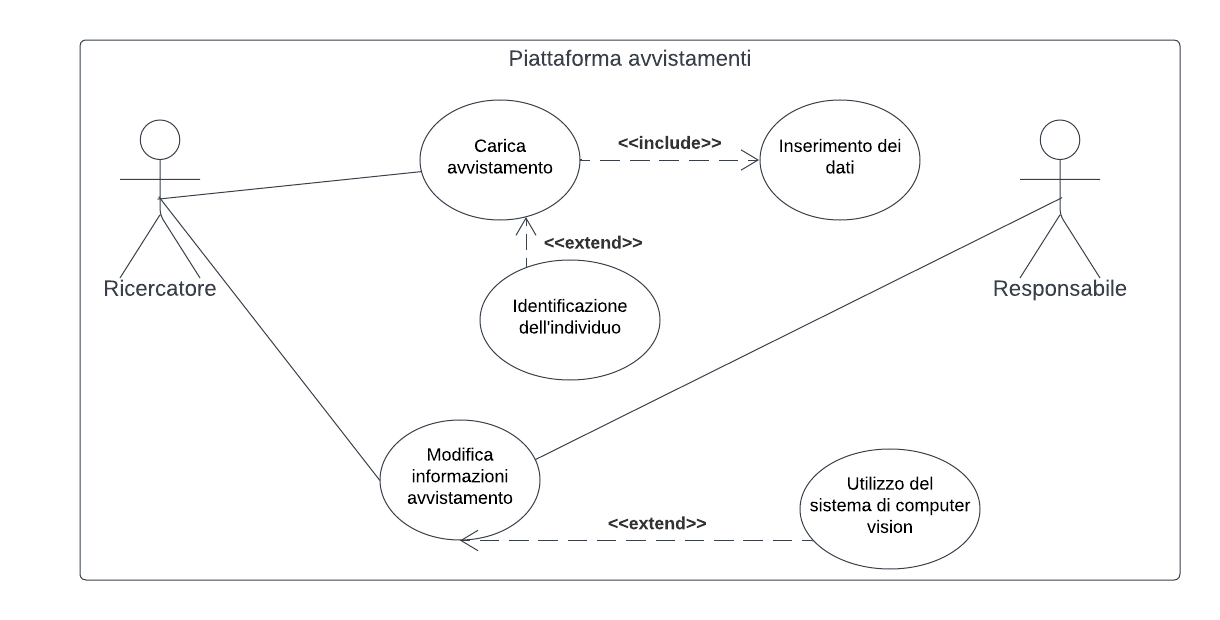
\includegraphics[scale=0.6]{img_concettuale/casi.png}
\caption{Schema dei casi d'uso per la piattaforma.}
\end{figure}


\chapter{Documentazione Base di dati}
\section{Analisi dei requisiti}
In questa sezione analizzeremo tutte le specifiche che il committente richiede per la piattaforma.

\subsection{Intervista}
Di seguito si riporta la prima intervista col committente:
"La facoltà di Acquacoltura e Igiene delle produzioni ittiche richiede un sistema informativo per la gestione di una banca dati al fine di permettere la registrazione di determinati avvistamenti durante le uscite a largo dalla costa.\\
Ogni utente, il quale ha a disposizione uno smartphone, una volta effettuato l'accesso con login e password, ha la possibilità di inserire un nuovo avvistamento, per il quale gli elementi da memorizzare sono la data e ora corrente(inserite in autonomia dal sistema), il numero di esemplari che sono stati avvistati e opzionalmente anche il vento in km/h, le condizioni del mare, eventuali ferite visibili. In particolare si ponga attenzione alla descrizione della ferita, la sua posizione e la relativa gravità. Deve anche essere possibile scrivere note che possano aiutare ad individuare la specie e/o elementi che aggiungano informazioni all'avvistamento. 
\\
Un avvistamento può far riferimento ad un particolare animale, a una specie specifica o anche a nessuna delle due: il terzo caso viene preso in considerazione quando chi sta eseguendo la rilevazione non ha la possibilità di riconoscere la specie esatta, inseribile comunque in un secondo momento.
\\
Oltre all'applicazione smartphone deve essere realizzato un applicativo web il quale, una volta effettuato l'accesso, deve poter visualizzare tutti gli avvistamenti che sono stati effettuati dagli utenti e poter modificare i parametri. La modifica deve essere permessa per tutti i dati, eccetto gli elementi che riguardo l'utente e la data della rilevazione.
\\ 
Ad ogni avvistamento il personale addetto può associare anche una o più immagini. Esse serviranno in seguito per il riconoscimento della specie di appartenenza. Dato che in un avvistamento possono essere presenti anche più animali, comunque tutti della stessa specie, la foto può essere suddivisa in più parti in modo tale da isolare ogni singolo individuo.
\\
La base di dati deve anche tenere in considerazione la possibilità di avvistamenti dello stesso individuo in momenti diversi. Nello specifico, attraverso le sottoimmagini se si avvista più volte lo stesso esemplare si deve avere la possibilità di associargli entrambe le immagini riferite a lui, in modo tale da vedere la sua evoluzione nel tempo.
\\
Per aiutare l'utente nella decisione della specie da assegnare a un particolare animale, il sistema deve memorizzare una descrizione, in cui vengono fornite le informazioni base su ciascuna specie analizzabile.
\\
Infine l'applicativo web, attraverso l'uso di visione artificiale ed in particolare per l'animale denominato delfino, deve poter essere in grado in autonomia di identificare la relativa specie attraverso la foto scattata durante il rilevamento. Nello specifico deve cercare di aiutare l'utente nella scelta della specie, stilando una classifica di compatibilità con le specie che ha presenti in database.
\\
Un aspetto importante da tenere in considerazione è il fatto che il sistema in autonomia, siccome se ci si trova a largo della costa non è presente connessione, deve poter lo stesso mantenere i dati in memoria e caricali una volta che ha la possibilità di farlo".

\subsection{Rilevamento delle ambiguità e correzioni proposte}
Il testo dell'intervista presenta molte ambiguità. Le principali sono:
\begin{itemize}
\item Utilizzo di sinonimi.
\item Elenchi di attributi incompleti.
\item Cardinalità non specificate.
\end{itemize}

Per quanto riguarda gli attributi parziali e le cardinalità, questi aspetti saranno corretti mediante l'uso della logica in fase di creazione dello schema concettuale. Invece per quanto concerne i sinonimi, è necessario costruire un glossario dei termini, i quali saranno considerati al fine della progettazione concettuale:

\begin{table}[hbtp]
\centering
\resizebox{10cm}{!}{%
\begin{tabular}{|c|c|c|c|}
\hline
\cellcolor[HTML]{C0C0C0} Termine & \cellcolor[HTML]{C0C0C0}  Descrizione & \cellcolor[HTML]{C0C0C0} Sinonimi & \cellcolor[HTML]{C0C0C0} Collegamenti \\ \hline
Utente & \begin{tabular}[c]{@{}c@{}}Persona che accede\\  al portale al fine \\ di inserire un\\  nuovo avvistamento\\  oppure per modificare\\  avvistamenti\\  già presenti \\ nella banca dati\end{tabular} & Persona & Avvistamento \\ \hline
Avvistamento & \begin{tabular}[c]{@{}c@{}}Avvistamento di\\ un esemplare, al\\ fine di memorizzare\\ informazioni\end{tabular} & Rilevazione & \begin{tabular}[c]{@{}c@{}}Utente\\ Animale\\ Specie\\ Immagine\end{tabular} \\ \hline
Animale & \begin{tabular}[c]{@{}c@{}}Tipologia di \\ animale\\ avvistato\end{tabular} & Specie marina & \begin{tabular}[c]{@{}c@{}}Avvistamento\\ Specie\end{tabular} \\ \hline
Specie & \begin{tabular}[c]{@{}c@{}}Specie dell'animale\\ avvistato\end{tabular} &  & \begin{tabular}[c]{@{}c@{}}Animale\\ Avvistamento\\ Descrizione\end{tabular} \\ \hline
Descrizione & \begin{tabular}[c]{@{}c@{}}Descrizione specifica\\ al fine di una migliore\\ selezione della specie\end{tabular} &  & Specie \\ \hline
Immagine & \begin{tabular}[c]{@{}c@{}}Immagine \\ che rappresenta\\ l'avvistamento\end{tabular} & Foto & \begin{tabular}[c]{@{}c@{}}Avvistamento\\ Sottoimmagine\end{tabular} \\ \hline
Sottoimmagine & \begin{tabular}[c]{@{}c@{}}Sezioni di immagini\\ dei singoli individui\end{tabular} &  & \begin{tabular}[c]{@{}c@{}}Immagine\\ Ferita\\ Esemplare\end{tabular} \\ \hline
Ferita & \begin{tabular}[c]{@{}c@{}}Ferita sul corpo di \\ un animale, con una \\ gravità\end{tabular} &  & Sottoimmagine \\ \hline
Esemplare & \begin{tabular}[c]{@{}c@{}}Singolo animale\\ che si monitora\end{tabular} &  & Sottoimmagine \\ \hline
\end{tabular}%
}
\end{table}

\newpage

\subsection{Estrazione dei concetti principali}
Dall'intervista si ricavano anche le operazioni principali richieste:
\begin{itemize}
\item Creazione di un nuovo utente.
\item Registrazione di un nuovo avvistamento attraverso l'applicazione mobile.
\item Inserimento di ferite riconducibili al singolo animale con specifica della gravità.
\item Possibilità di inserimento di una o più immagini dell'avvistamento.
\item Possibilità di visualizzare, modificare ed eliminare un avvistamento.
\item Possibilità di suddividere immagini in più parti, e ciascuna delle quali a seconda dell'animale analizzarla attraverso un sistema di riconoscimento della specie.
\item Monitorare gli avvistamenti di particolari individui al fine di determinate verifiche.
\item Possibilità di consultazione di informazioni relative alla specie che si vuole attribuire a un determinato animale, al fine di una selezione più accurata.
\item Caricamento del nuovo avvistamento, compreso di dati e immagini anche in un secondo momento, nel caso non sia presente connessione.
\end{itemize}

\section{Progettazione Concettuale}
La fase di progettazione concettuale consiste parzialmente nella formalizzazione dei requisiti, in particolare sui termini e sulle transazioni, i quali sono stati raccolti e analizzati nella fase precedente.

\subsection{Schema scheletro}
Per maggiore chiarezza, di seguito riportiamo i primi esempi di schemi concettuali divisi per ambiti.

\begin{figure}[hbtp]
\centering
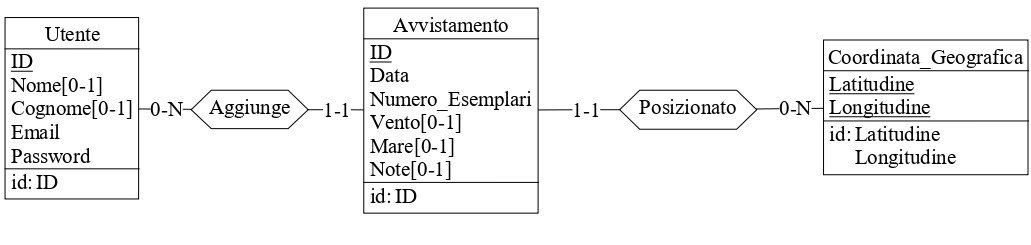
\includegraphics[scale=0.15]{img_concettuale/avvistamento1.png}
\caption{Schema concettuale per la modellazione degli avvistamenti e delle proprietà dell'utente.}
\end{figure}

Come mostrato in figura sono presenti uno o più utenti, ognuno dei quali accedono alla piattaforma attraverso la propria email, password e grazie a una chiave personale univoca all'interno del database, la quale viene utilizzata al fine di criptare la password. Di tale utente possiamo tenere anche in considerazione il proprio nome e cognome.
Ogni utente aggiunge degli avvistamenti, ognuno dei quali contiene tutti i dati richiesti del committente tra cui la data di avvistamento, il numero di esemplari presenti e opzionalmente anche il vento espresso in km/h, lo stato del mare ed eventuali note informative al fine di ricerca e in particolare per riuscire ad identificare meglio la specie.\\
In aggiunta per ogni avvistamento è associata una posizione la quale tiene in considerazione la longitudine e la latitudine al momento dell'inserimento.

\begin{figure}[hbtp]
\centering
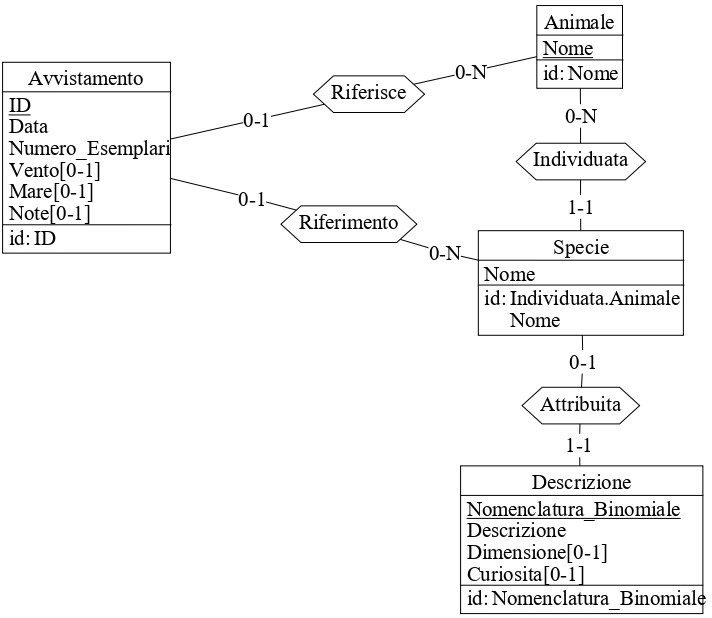
\includegraphics[scale=0.10]{img_concettuale/avvistamento2.png}
\caption{Modellazione dell'attribuzione dell'animale e della specie all' avvistamento.}
\end{figure}

Dalla figura si può notare che un avvistamento può far riferimento a un animale, direttamente alla specie o anche a nessuno dei due, in quest'ultimo caso tali dati verranno inseriti in un secondo momento. Al fine di individuare al meglio la specie ad ognuna può essere attribuita una descrizione in cui vengono elencate le caratteristiche fondamentali. Ogni specie è identificata dal nome dell'animale e dal suo nome specifico. Come si nota dalla figura, l'avvistamento può essere direttamente associato all'animale oppure alla specie, in questo caso nasce il vincolo che se dichiaro una determinata specie essa deve fare  riferimento al giusto animale. Un ulteriore vincolo da rispettare è il fatto che in un avvistamento, anche se esso include più esemplari, questi devono far riferimento allo stesso animale ed eventualmente alla relativa specie.

\begin{figure}[hbtp]
\centering
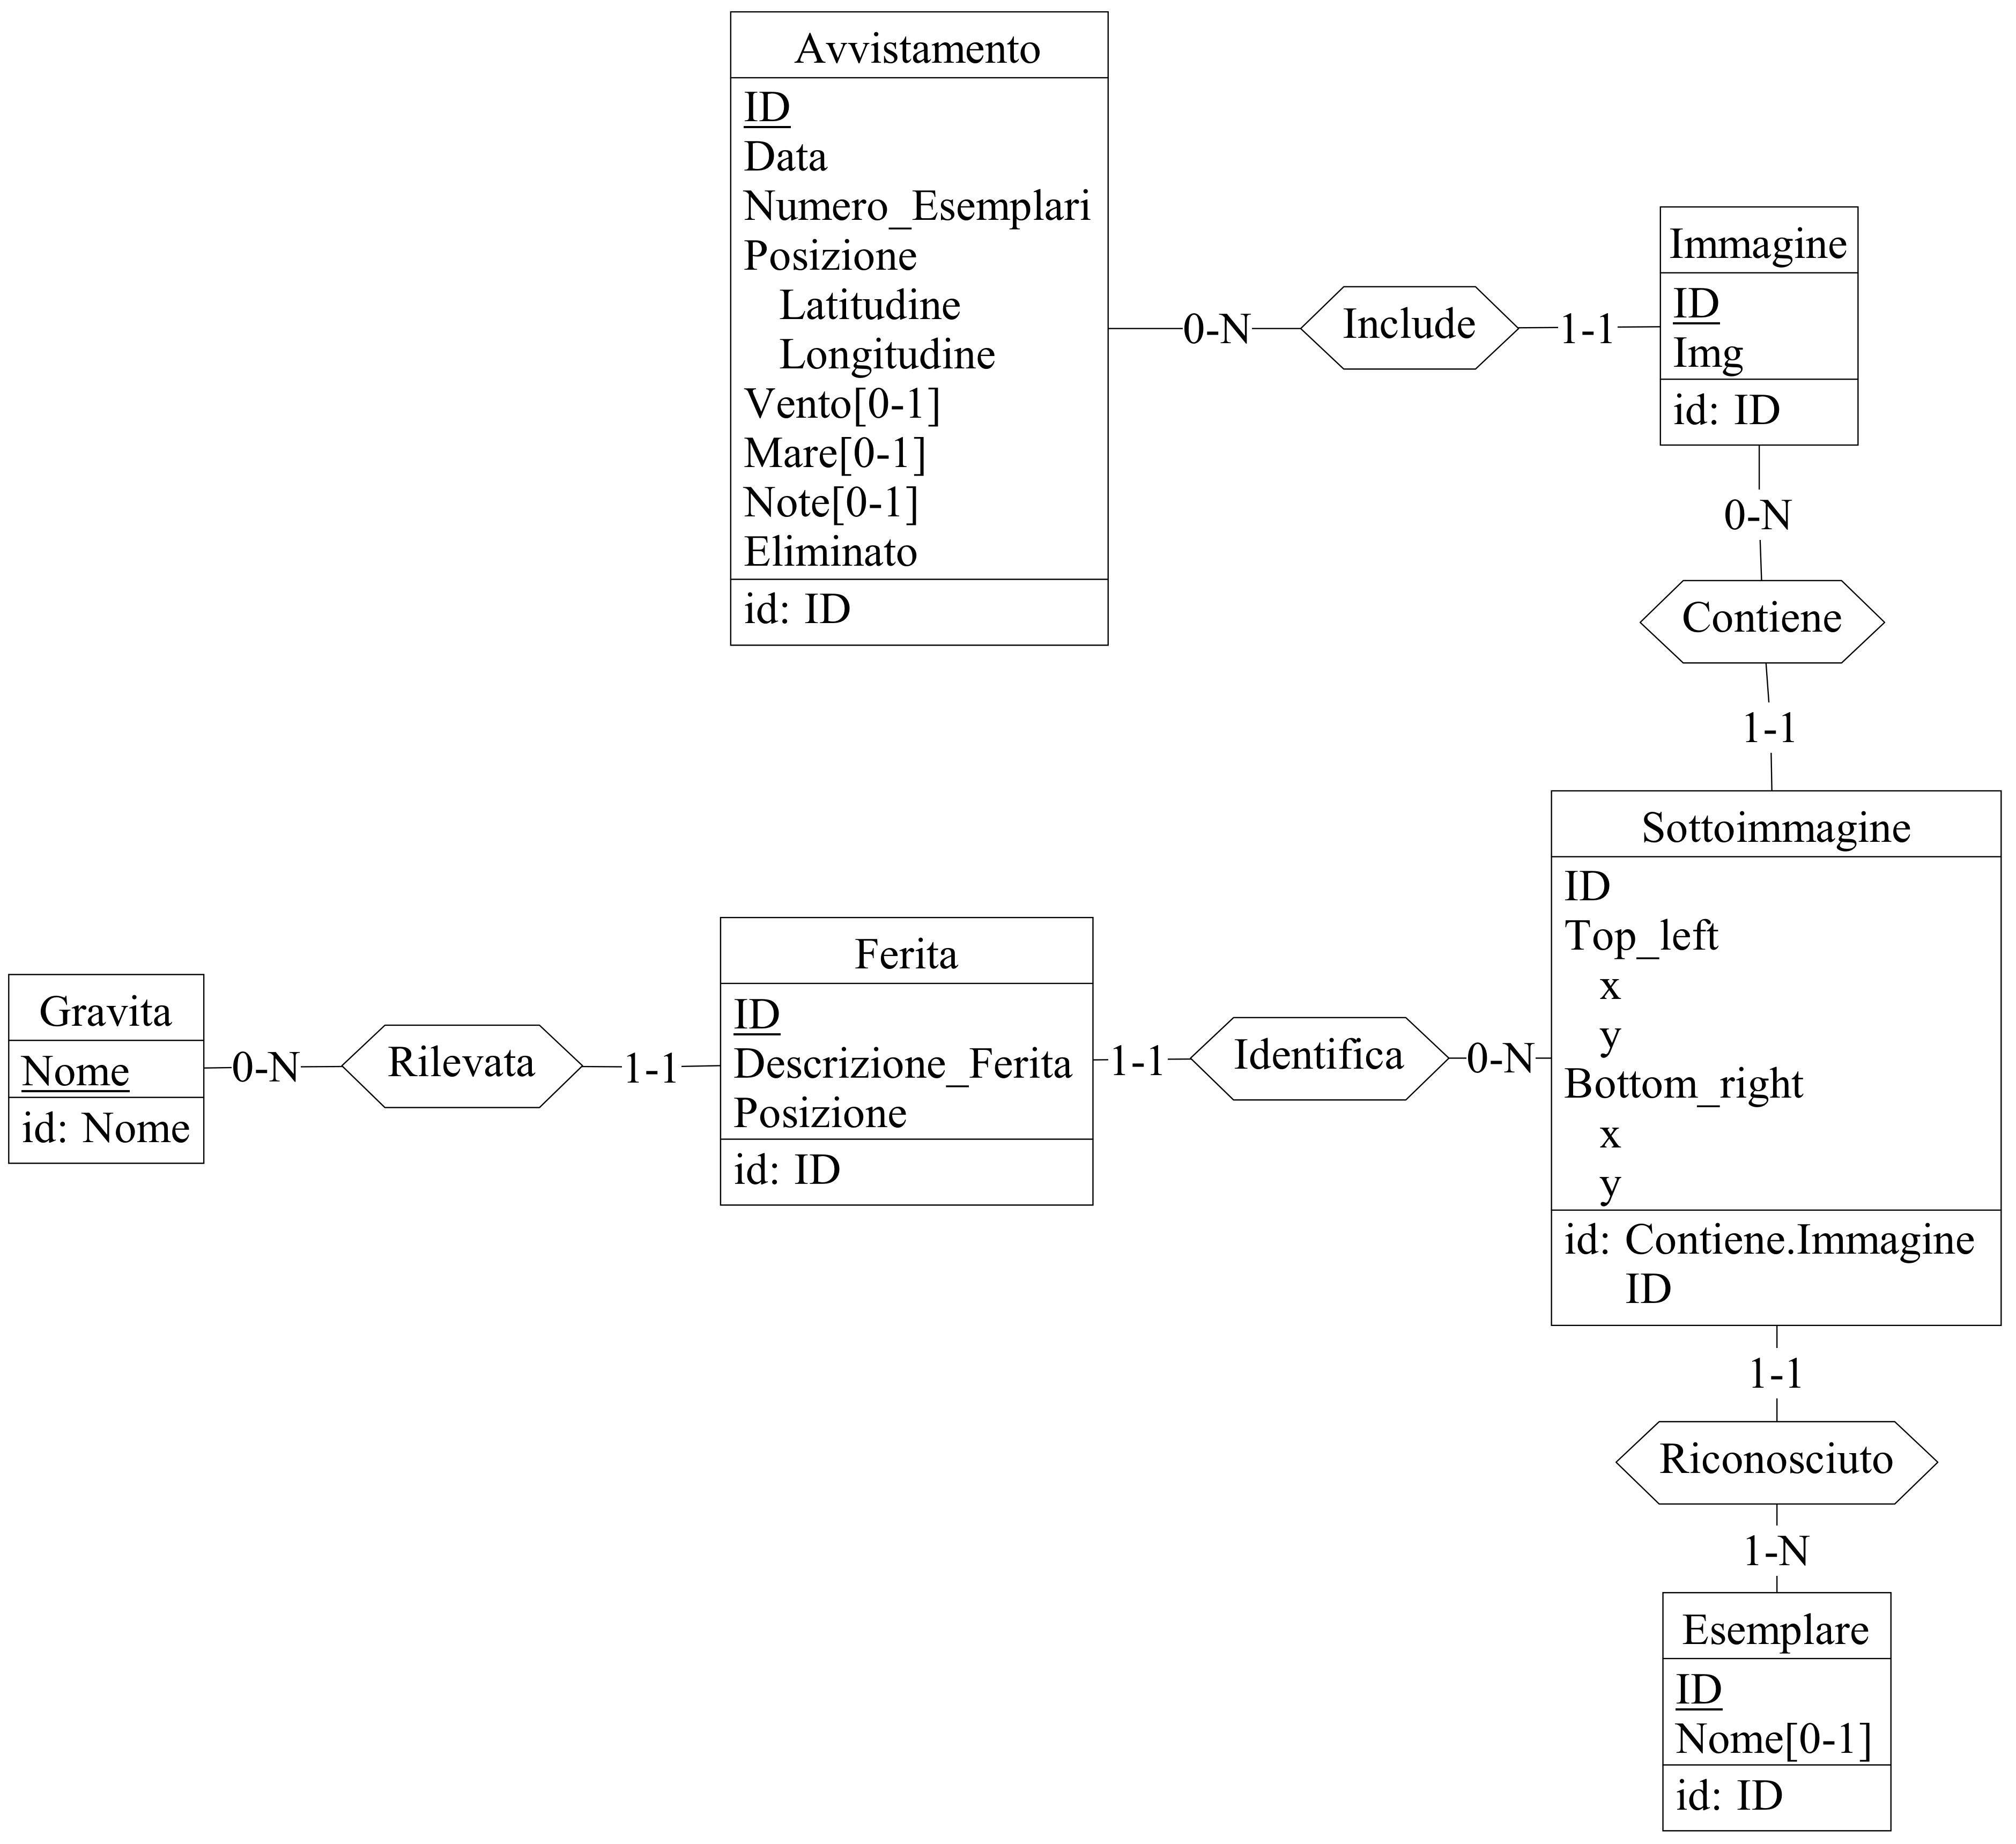
\includegraphics[scale=0.13]{img_concettuale/avvistamento3.png}
\caption{Schema concettuale raffigurante le immagini con relative sottoimmagini e la gestione delle ferite.}
\end{figure}

Navigando lo schema partendo dall'entità Avvistamento, si nota che per ogni avvistamento si possono includere una o più immagini le quali possono essere suddivise in ulteriori sottoimmagini, per fare questo si è pensato di utilizzare le coordinate cartesiane al fine di risparmiare memoria e tempo di elaborazione. Visto che ogni sottoimmagine rappresenta un elemento singolo, se esso presenta delle ferite queste possono essere inserite e ad ognuna attribuita una gravità. In aggiunta il singolo individuo viene catalogato, con un id e opzionalmente anche con un nome, in modo tale che se viene rincontrato in altri avvistamenti si abbia la possibilità di indicare che si tratta dello stesso esemplare.

\subsection{Raffinamenti attuati}
Elenchiamo in questa sezione i raffinamenti che sono stati attuati nei precedenti schemi al fine di modellare meglio entità indipendenti. In particolare:
\begin{itemize}
\item L'entità Descrizione è stata creata al fine di non appesantire troppo l'entità Specie con attributi opzionali, i quali come si vede dallo schema rappresentano alla fine una sezione a parte del dominio. 
\end{itemize}

\subsection{Schema concettuale finale}
Di seguito si riporta lo schema concettuale finale, ottenuto unendo opportunamente gli schemi scheletro presentati in precedenza.
\newpage
\begin{figure}[hbtp]
\centering
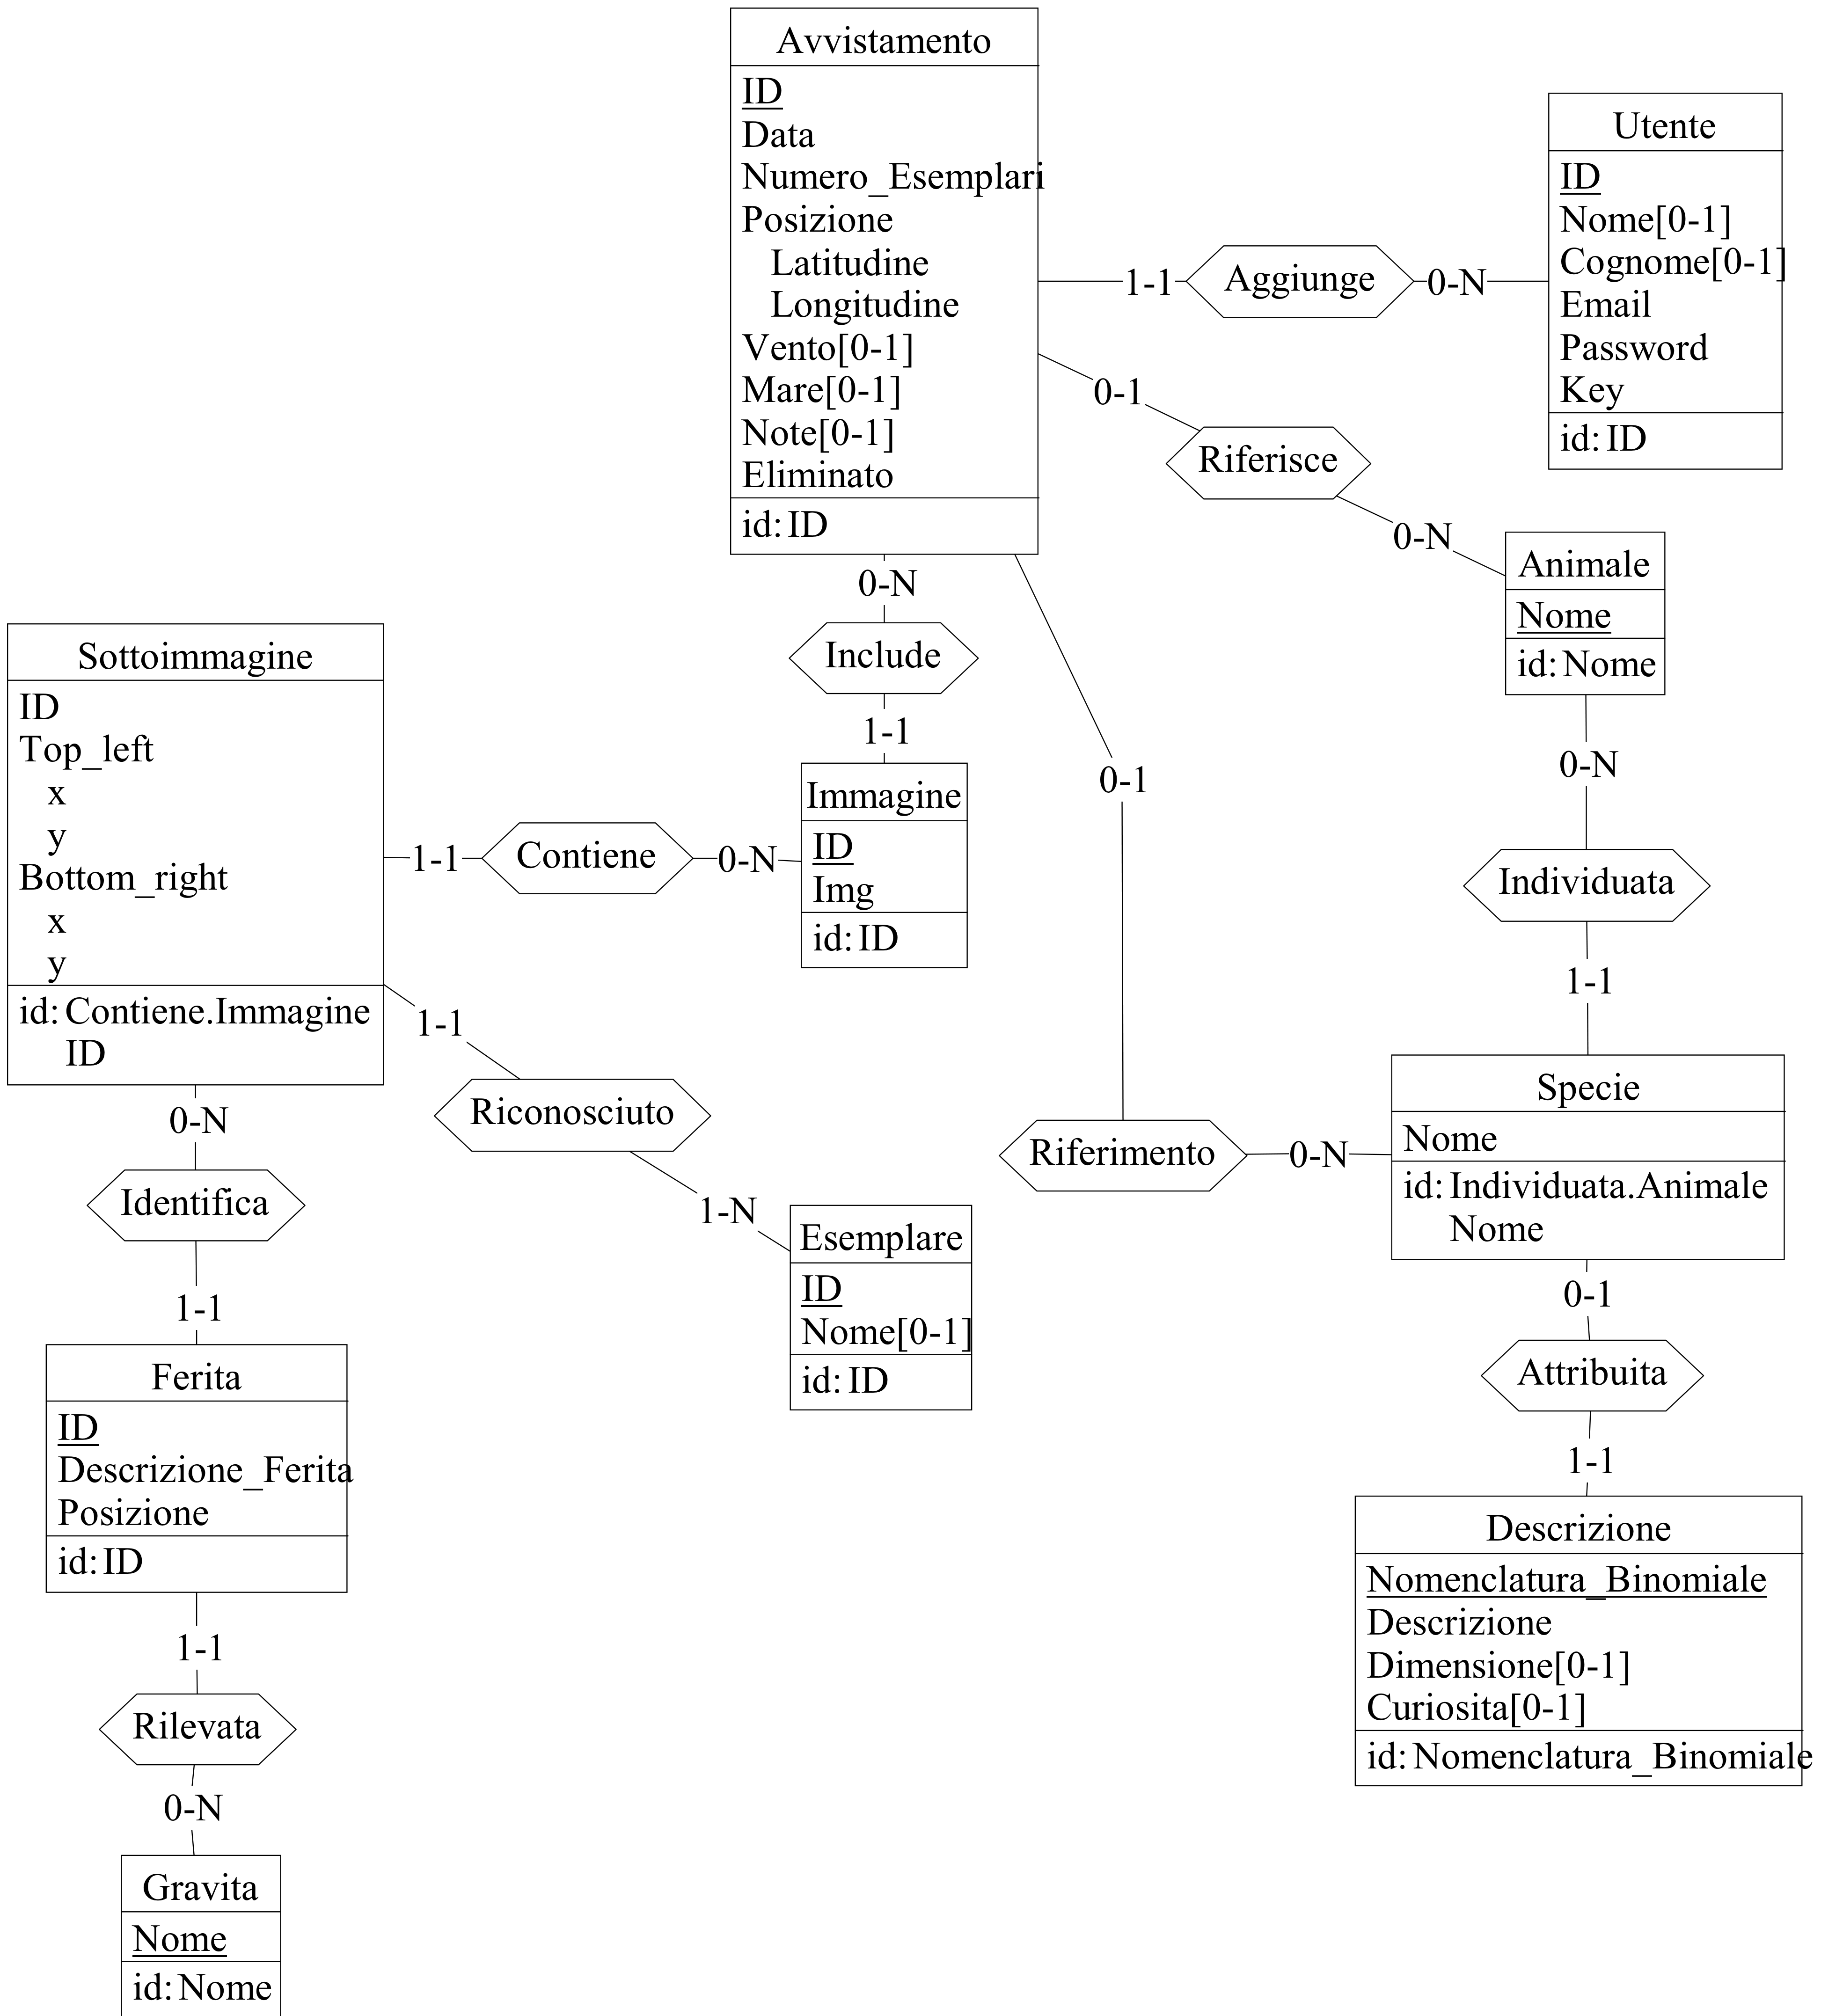
\includegraphics[scale=0.1]{img_concettuale/ER2.png}
\caption{Schema concettuale finale}
\end{figure}



\section{Progettazione Logica}
La progettazione logica consiste nella traduzione dello schema concettuale finale in uno schema logico che rispecchi il modello relazionale. Lo schema logico progettato è indipendente dallo specifico Database management system, che verrà scelto al termine della progettazione logica. Inoltre verranno definiti anche i vincoli di integrità sui dati.

\subsection{Stima del volume dei dati}
Nella tabella di seguito è riportato il volume atteso per ciascun costrutto presente nello schema concettuale.
Inoltre, per garantire maggiore compattezza, sono state omesse le stime dei volumi delle associazioni 1-N, in quanto equivalenti ai volumi delle entità che partecipano alle associazioni stesse con cardinalità 1.

\begin{table}[hbtp]
\centering
\begin{tabular}{|c|c|c|}
\hline
\rowcolor[HTML]{C0C0C0} 
{\color[HTML]{000000} Concetto} & {\color[HTML]{000000} Costrutto} & {\color[HTML]{000000} Volume} \\ \hline
Avvistamento           & E & 100 \\ \hline
Utente                 & E & 10  \\ \hline
Immagine               & E & 200 \\ \hline
Sottoimmagine          & E & 400 \\ \hline
Ferita                 & E & 50  \\ \hline
Gravita                & E & 3   \\ \hline
Esemplare              & E & 300 \\ \hline
Animale                & E & z   \\ \hline
Specie                 & E & x   \\ \hline
Descrizione            & E & x-y \\ \hline
\end{tabular}
\end{table}

\subsection{Descrizione delle operazioni principali e stima della loro frequenza}
Di seguito si riporta una tabella contenente la frequenza prevista e una descrizione delle principali operazioni, individuate già in fase di analisi.
\begin{table}[hbtp]
\centering
\resizebox{\columnwidth}{!}{%
\begin{tabular}{|c|c|c|}
\hline
\rowcolor[HTML]{C0C0C0} 
{\color[HTML]{000000} Codice Operazione} & {\color[HTML]{000000} Descrizione Operazione} & {\color[HTML]{000000} Frequenza} \\ \hline
{\color[HTML]{000000} 1} & {\color[HTML]{000000} Creazione di un nuovo utente} & {\color[HTML]{000000} 1/settimana} \\ \hline
{\color[HTML]{000000} 2} & {\color[HTML]{000000} \begin{tabular}[c]{@{}c@{}}Monitoraggio di specifici individui\end{tabular}} & {\color[HTML]{000000} 5/giorno} \\ \hline
{\color[HTML]{000000} 3} & {\color[HTML]{000000} \begin{tabular}[c]{@{}c@{}}Registrazione di un nuovo avvistamento\\ compreso di operazioni opzionali\end{tabular}} & {\color[HTML]{000000} 10/giorno} \\ \hline
\end{tabular}%
}
\end{table}

\subsection{Schemi di navigazione e tabelle degli accessi}
Dopo aver stimato i volumi dei principali costrutti presenti nella base di dati e la 
frequenza delle principali operazioni, si può procedere a disegnare i relativi schemi 
di navigazione e scrivere le tabelle degli accessi.

\begin{enumerate}
\item Creazione di un nuovo utente:\\
Per quanto riguarda l'aggiunta dell'utente, omettiamo il corrispondente schema di navigazione in quanto coincide con l'entità stessa:

\begin{table}[hbtp]
\centering
\resizebox{7cm}{!}{%
\begin{tabular}{|c|ccl|}
\hline
\rowcolor[HTML]{C0C0C0} 
{\color[HTML]{000000} Concetto} &
  \multicolumn{1}{c|}{\cellcolor[HTML]{C0C0C0}{\color[HTML]{000000} Costrutto}} &
  \multicolumn{1}{c|}{\cellcolor[HTML]{C0C0C0}{\color[HTML]{000000} Accessi}} &
  Tipo \\ \hline
Utente &
  \multicolumn{1}{c|}{E} &
  \multicolumn{1}{c|}{1} &
  S \\ \hline
 &
  \multicolumn{3}{c|}{Totale = 1S} \\ \hline
\end{tabular}%
}
\end{table}

\newpage

\item Monitoraggio di specifici individui al fine di determinate verifiche:
\begin{figure}[hbtp]
\centering
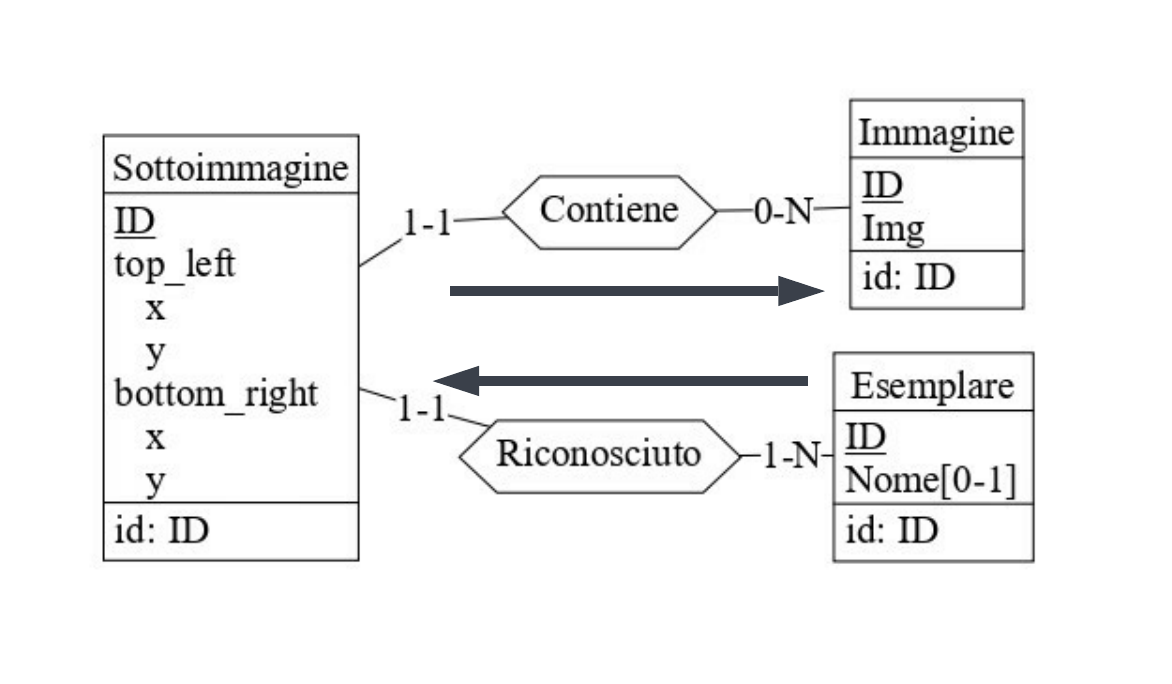
\includegraphics[scale=1.1]{img_concettuale/individuo.png}
%\caption{Schema concettuale raffigurante gli accessi alle tabelle per il monitoraggio di specifici individui.}
\end{figure}
\\Per svolgere questa operazione occorre effettuare un totale di letture su Sottoimmagine pari al numero medio di foto a cui ogni esemplare è associato. In aggiunta, in base al numero di sottoimmagini a cui l'esemplare è associato si dovranno selezionare lo stesso numero di immagini, visto che uno stesso esemplare non può comparire più volte nella stessa immagine.
\begin{table}[hbtp]
\centering
\resizebox{11cm}{!}{%
\begin{tabular}{|c|ccc|}
\hline
\rowcolor[HTML]{C0C0C0} 
{\color[HTML]{000000} Concetto} &
  \multicolumn{1}{c|}{\cellcolor[HTML]{C0C0C0}{\color[HTML]{000000} Costrutto}} &
  \multicolumn{1}{c|}{\cellcolor[HTML]{C0C0C0}{\color[HTML]{000000} Accessi}} &
  {\color[HTML]{000000} Tipo} \\ \hline
{\color[HTML]{000000} Esemplare}     & \multicolumn{1}{c|}{{\color[HTML]{000000} E}} & \multicolumn{1}{c|}{{\color[HTML]{000000} 1}}         & {\color[HTML]{000000} L} \\ \hline
{\color[HTML]{000000} Sottoimmagine} & \multicolumn{1}{c|}{{\color[HTML]{000000} E}} & \multicolumn{1}{c|}{{\color[HTML]{000000} 400$\div$200=2}} & {\color[HTML]{000000} L} \\ \hline
Immagine                             & \multicolumn{1}{c|}{E}                        & \multicolumn{1}{c|}{2}                                & L                        \\ \hline
                                     & \multicolumn{3}{c|}{Totale = 5L}                                                                                                 \\ \hline
\end{tabular}%
}
\end{table}

\newpage
\item Registrazione di un nuovo avvistamento compreso di operazioni opzionali:
\begin{figure}[hbtp]
\centering
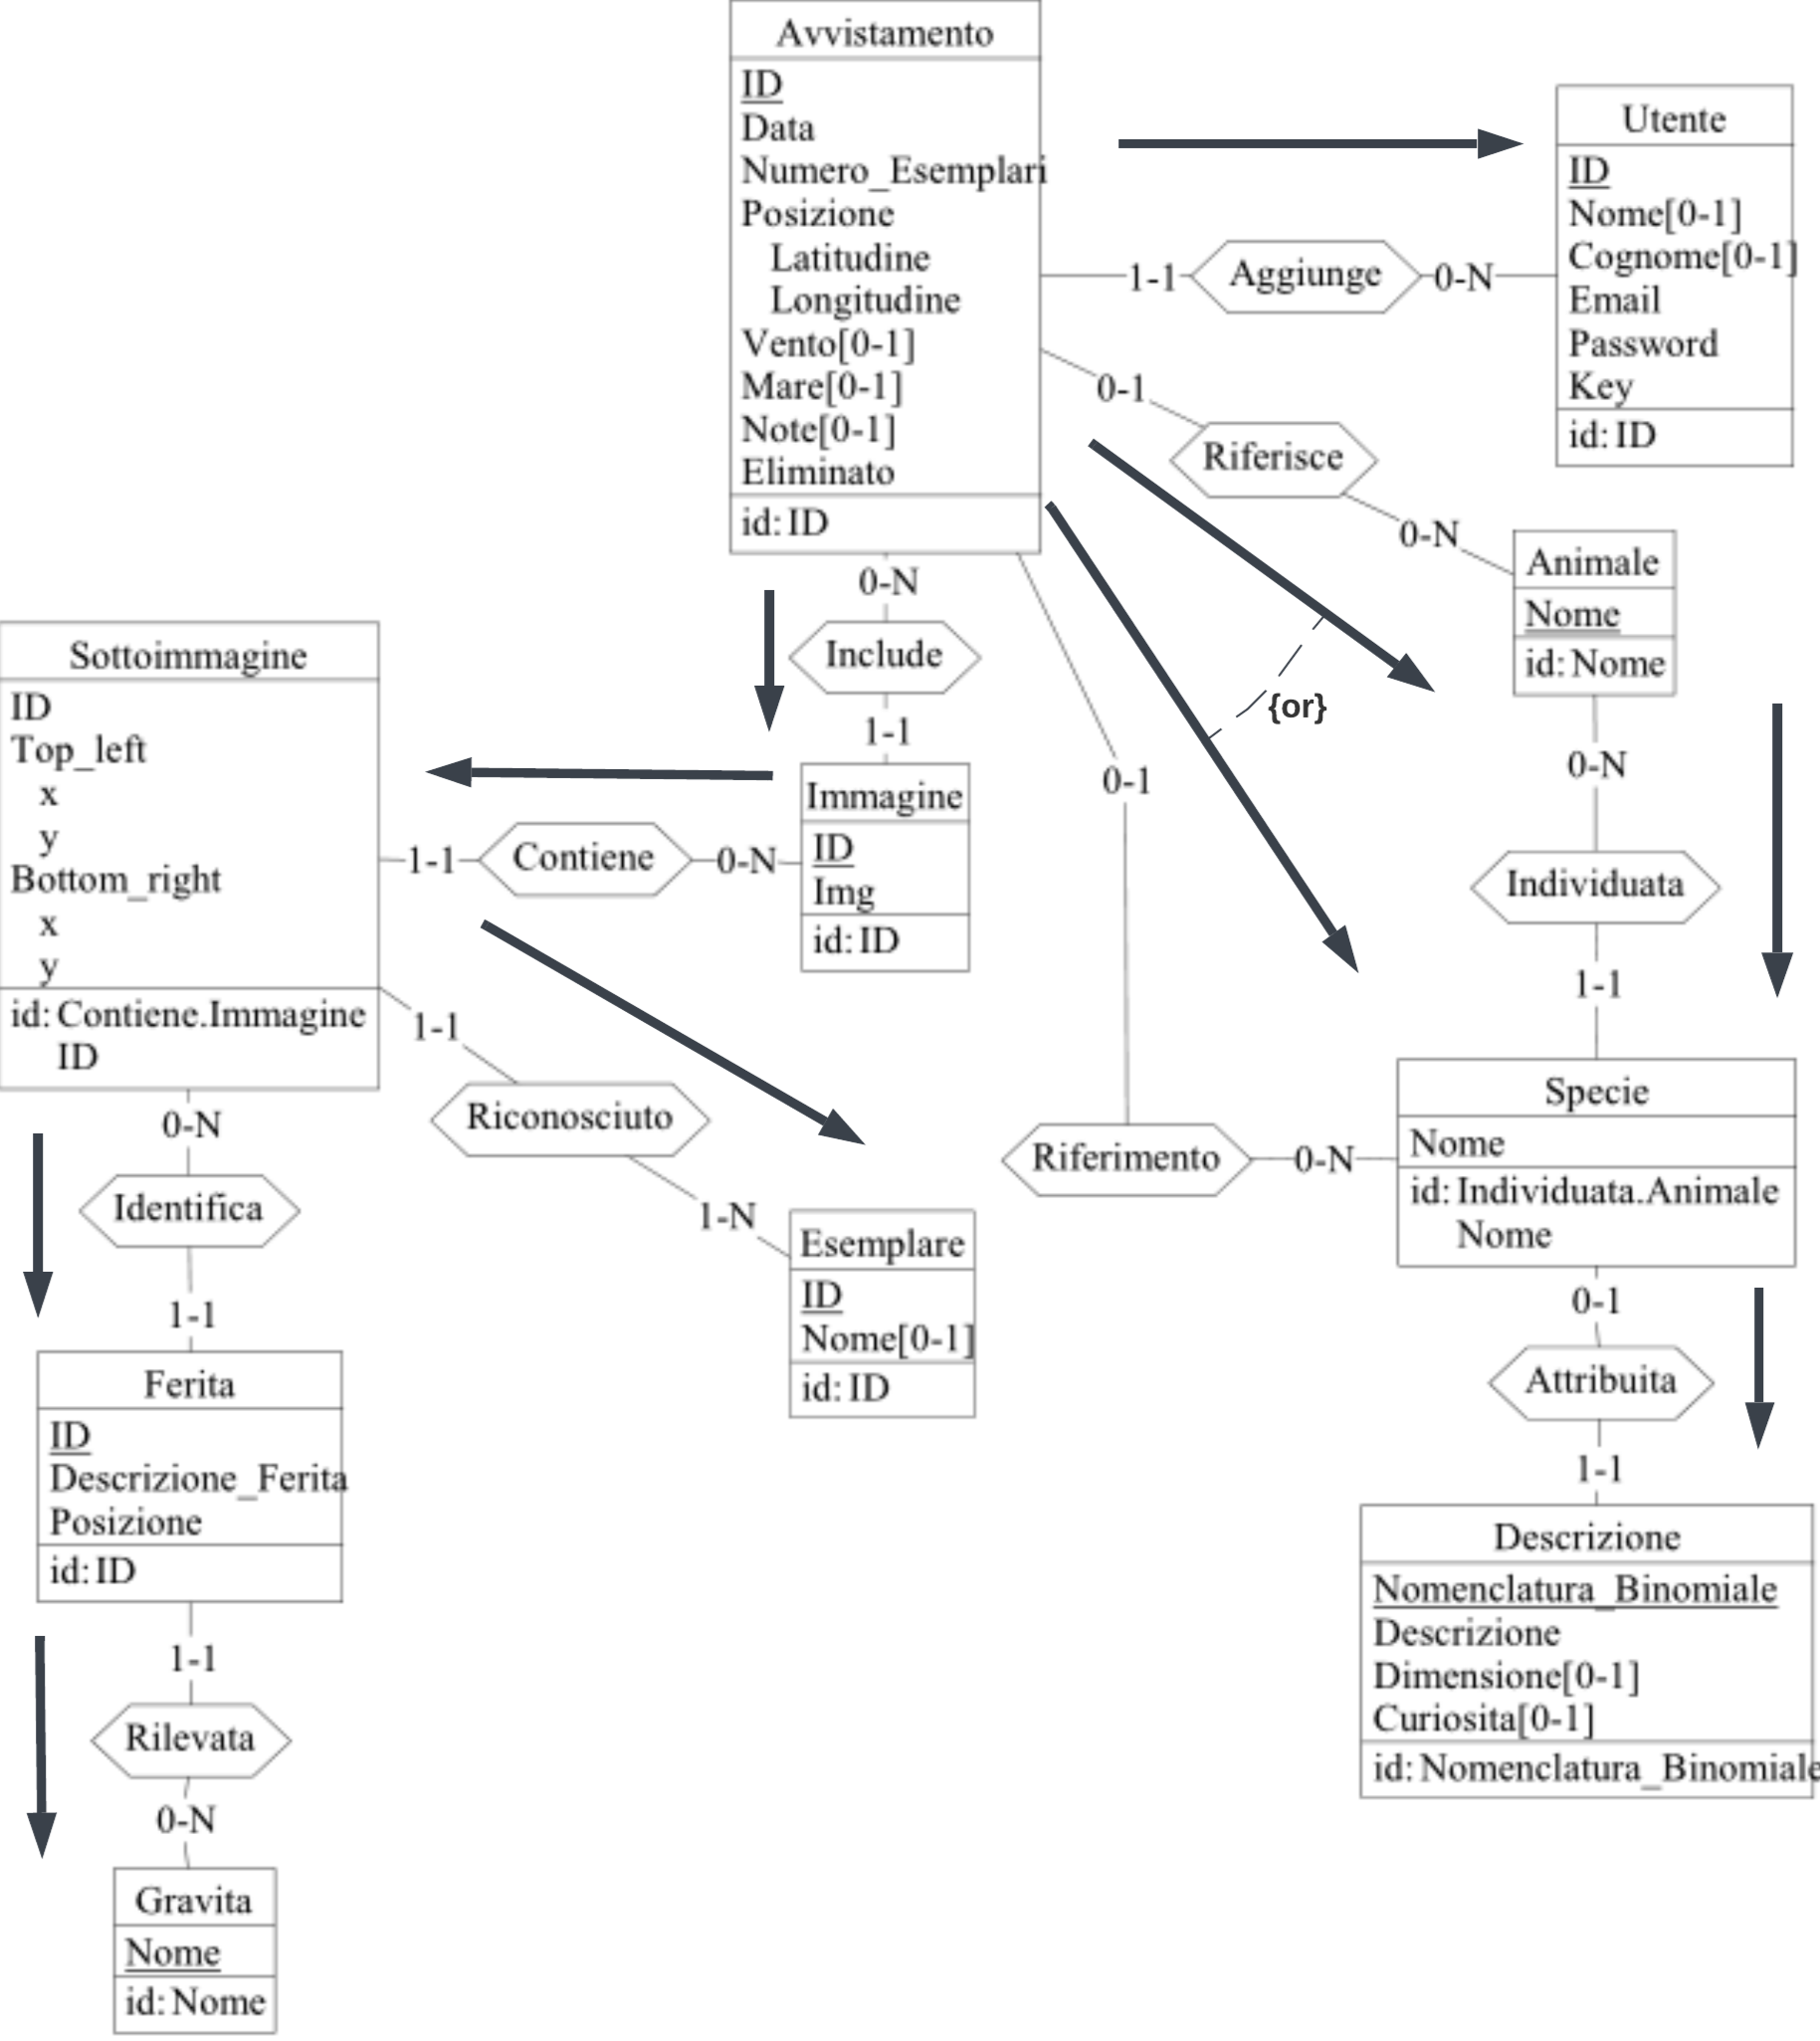
\includegraphics[scale=0.20]{img_concettuale/Avvistamento_accessi.png}
\caption{Schema concettuale raffigurante gli accessi alle tabelle per l'aggiunta di un nuovo avvistamento.}
\end{figure}\\
Lo schema di navigazione prevede di partire da Avvistamento, il quale legge l'utente, poi aggiunge più immagini le quali verranno suddivise in più sottoimmagini, ad ognuna delle quali verrà associato un esemplare. In aggiunta, ad ogni sottoimmagine si possono aggiungere delle possibili ferite, visibili in quella parte dell'immagine, ad ogni ferita è obbligatorio associargli una gravità. Nella tabella degli accessi sottostante consideriamo il caso in cui l'esemplare e la coordinata geografica non siano ancora presenti nel database. Ogni avvistamento è associato ad un'animale e di conseguenza a una possibile specie. Al fine di individuare meglio la specie, essa è associata a una possibile descrizione.\\ Un'alternativa è la possibilità di scegliere direttamente la specie partendo dall'avvistamento, ma questo viene considerato un caso raro.
\begin{table}[hbtp]
\centering
\resizebox{11cm}{!}{%
\begin{tabular}{|c|ccc|}
\hline
\rowcolor[HTML]{C0C0C0} 
{\color[HTML]{000000} Concetto} & \multicolumn{1}{c|}{\cellcolor[HTML]{C0C0C0}{\color[HTML]{000000} Costrutto}} & \multicolumn{1}{c|}{\cellcolor[HTML]{C0C0C0}{\color[HTML]{000000} Accessi}} & {\color[HTML]{000000} Tipo} \\ \hline
{\color[HTML]{000000} Avvistamento} & \multicolumn{1}{c|}{{\color[HTML]{000000} E}} & \multicolumn{1}{c|}{{\color[HTML]{000000} 1}} & {\color[HTML]{000000} S} \\ \hline
{\color[HTML]{000000} Utente} & \multicolumn{1}{c|}{{\color[HTML]{000000} E}} & \multicolumn{1}{c|}{{\color[HTML]{000000} 1}} & {\color[HTML]{000000} L} \\ \hline
Animale & \multicolumn{1}{c|}{E} & \multicolumn{1}{c|}{1} & L \\ \hline
Specie & \multicolumn{1}{c|}{E} & \multicolumn{1}{c|}{1} & L \\ \hline
Descrizione & \multicolumn{1}{c|}{E} & \multicolumn{1}{c|}{1} & L \\ \hline
Immagine & \multicolumn{1}{c|}{E} & \multicolumn{1}{c|}{200$\div$100=2} & S \\ \hline
Sottoimmagine & \multicolumn{1}{c|}{E} & \multicolumn{1}{c|}{(400$\div$200)$\times$2=4} & S \\ \hline
Ferita & \multicolumn{1}{c|}{E} & \multicolumn{1}{c|}{(50$\div$400)$\times$4=0.5} & S \\ \hline
Gravita & \multicolumn{1}{c|}{E} & \multicolumn{1}{c|}{1} & L \\ \hline
Esemplare & \multicolumn{1}{c|}{E} & \multicolumn{1}{c|}{4} & S \\ \hline
 & \multicolumn{3}{c|}{Totale = 11.5S + 5L} \\ \hline
\end{tabular}%
}
\end{table}

\end{enumerate}

\subsubsection{Accessi totali}
Si riporta di seguito la tabella degli accessi totali per ogni operazione, considerando doppi gli accessi in scrittura:
\begin{table}[hbtp]
\centering
\resizebox{12cm}{!}{%
\begin{tabular}{|c|c|c|c|}
\hline
\rowcolor[HTML]{C0C0C0} 
{\color[HTML]{000000} Codice Operazione} & {\color[HTML]{000000} Accessi} & {\color[HTML]{000000} Frequenza} & Totale \\ \hline
{\color[HTML]{000000} 1} & {\color[HTML]{000000} 1S = 2} & {\color[HTML]{000000} 1/settimana} & 2/settimana \\ \hline
{\color[HTML]{000000} 2} & {\color[HTML]{000000} 5L = 5} & {\color[HTML]{000000} 5/giorno} & 25/giorno \\ \hline
{\color[HTML]{000000} 3} & {\color[HTML]{000000} 11.5S + 5L = 28} & {\color[HTML]{000000} 10/giorno} & 280/giorno \\ \hline
\end{tabular}%
}
\end{table}

\subsection{Raffinamento dello schema}
In questa sezione ci occuperemo del raffinamento dello schema concettuale in vista della realizzazione dello schema logico. In particolare, bisognerà concentrarsi sulla seguente operazione.

\begin{itemize}
\item \textbf{Modifica degli attributi multipli e composti:}\\
Una volta individuate le entità che contengono attributi multipli o composti, si provvede a modificarli. In particolare: \\ 
\begin{itemize}
\item Nell'entità Sottoimmagine gli attributi top\_left e bottom\_right formati da x e y vengono trasformati in singoli attributi.
\item Nell'entità Avvistamento l'attributo posizione viene scomposto in due singole attributi denominati Latitudine e Longitudine. 
\end{itemize}
\end{itemize}

\subsection{Traduzione di entità e associazioni in relazioni}
La traduzione delle entità in relazioni è automatica e non richiede particolari passaggi.\\
Per quanto riguarda invece le associazioni, bisogna effettuare diversi passaggi in base alla cardinalità:
\begin{itemize}
\item  Le associazioni 1-N vengono tradotte importando nell'entità che partecipa con cardinalità 1 la chiave dell'entità che partecipa con cardinalità N.
\item Le associazioni 1-1 vengono tradotte importando nell'entità ritenuta più corretta, in base ad opzionalità e operatività, la chiave dell'altra entità.
\end{itemize}

L'operazione di traduzione porta alla creazione dello schema logico:\\
\textbf{Gravita}(\underline{Nome})\\
\textbf{Ferite}(\underline{ID}, Descrizione\_Ferita, Posizione, Gravi\_Nome:Gravita, \\ \tab Sottoi\_ID:Sottoimmagini, Img\_rif:Immagini)\\
\textbf{Sottoimmagini}(\underline{ID}, tl\_x, tl\_y, br\_x, br\_y, Immag\_ID:Immagini,\\ \tab Esemp\_ID:Esemplari)\\
\textbf{Esemplari}(\underline{ID}, Nome*)\\
\textbf{Immagini}(\underline{ID}, Img, Avvis\_ID:Avvistamenti)\\
\textbf{Utenti}(\underline{ID}, Nome*, Cognome*, Email, Password, Key)\\
\textbf{Animali}(\underline{Nome})\\
\textbf{Specie}((\underline{Nome, Anima\_Nome:Animali}),\\ \tab Nomenclatura\_Binomiale*:Descrizioni)\\
\textbf{Descrizioni}(\underline{Nomenclatura\_Binomiale}, Descrizione, Dimensione*,\\ \tab Curiosita*)\\
\textbf{Avvistamenti}(\underline{ID}, Data, Numero\_Esemplari, Vento*, Mare*, Note*,\\ \tab Latid, Long, Utente\_ID:Utenti, Anima\_Nome*:Animali,\\ \tab (Specie\_anima\_Nome, Specie\_Nome)*:Specie, Eliminato)\\

\newpage
\subsection{Schema relazionale finale}
\begin{figure}[hbtp]
\centering
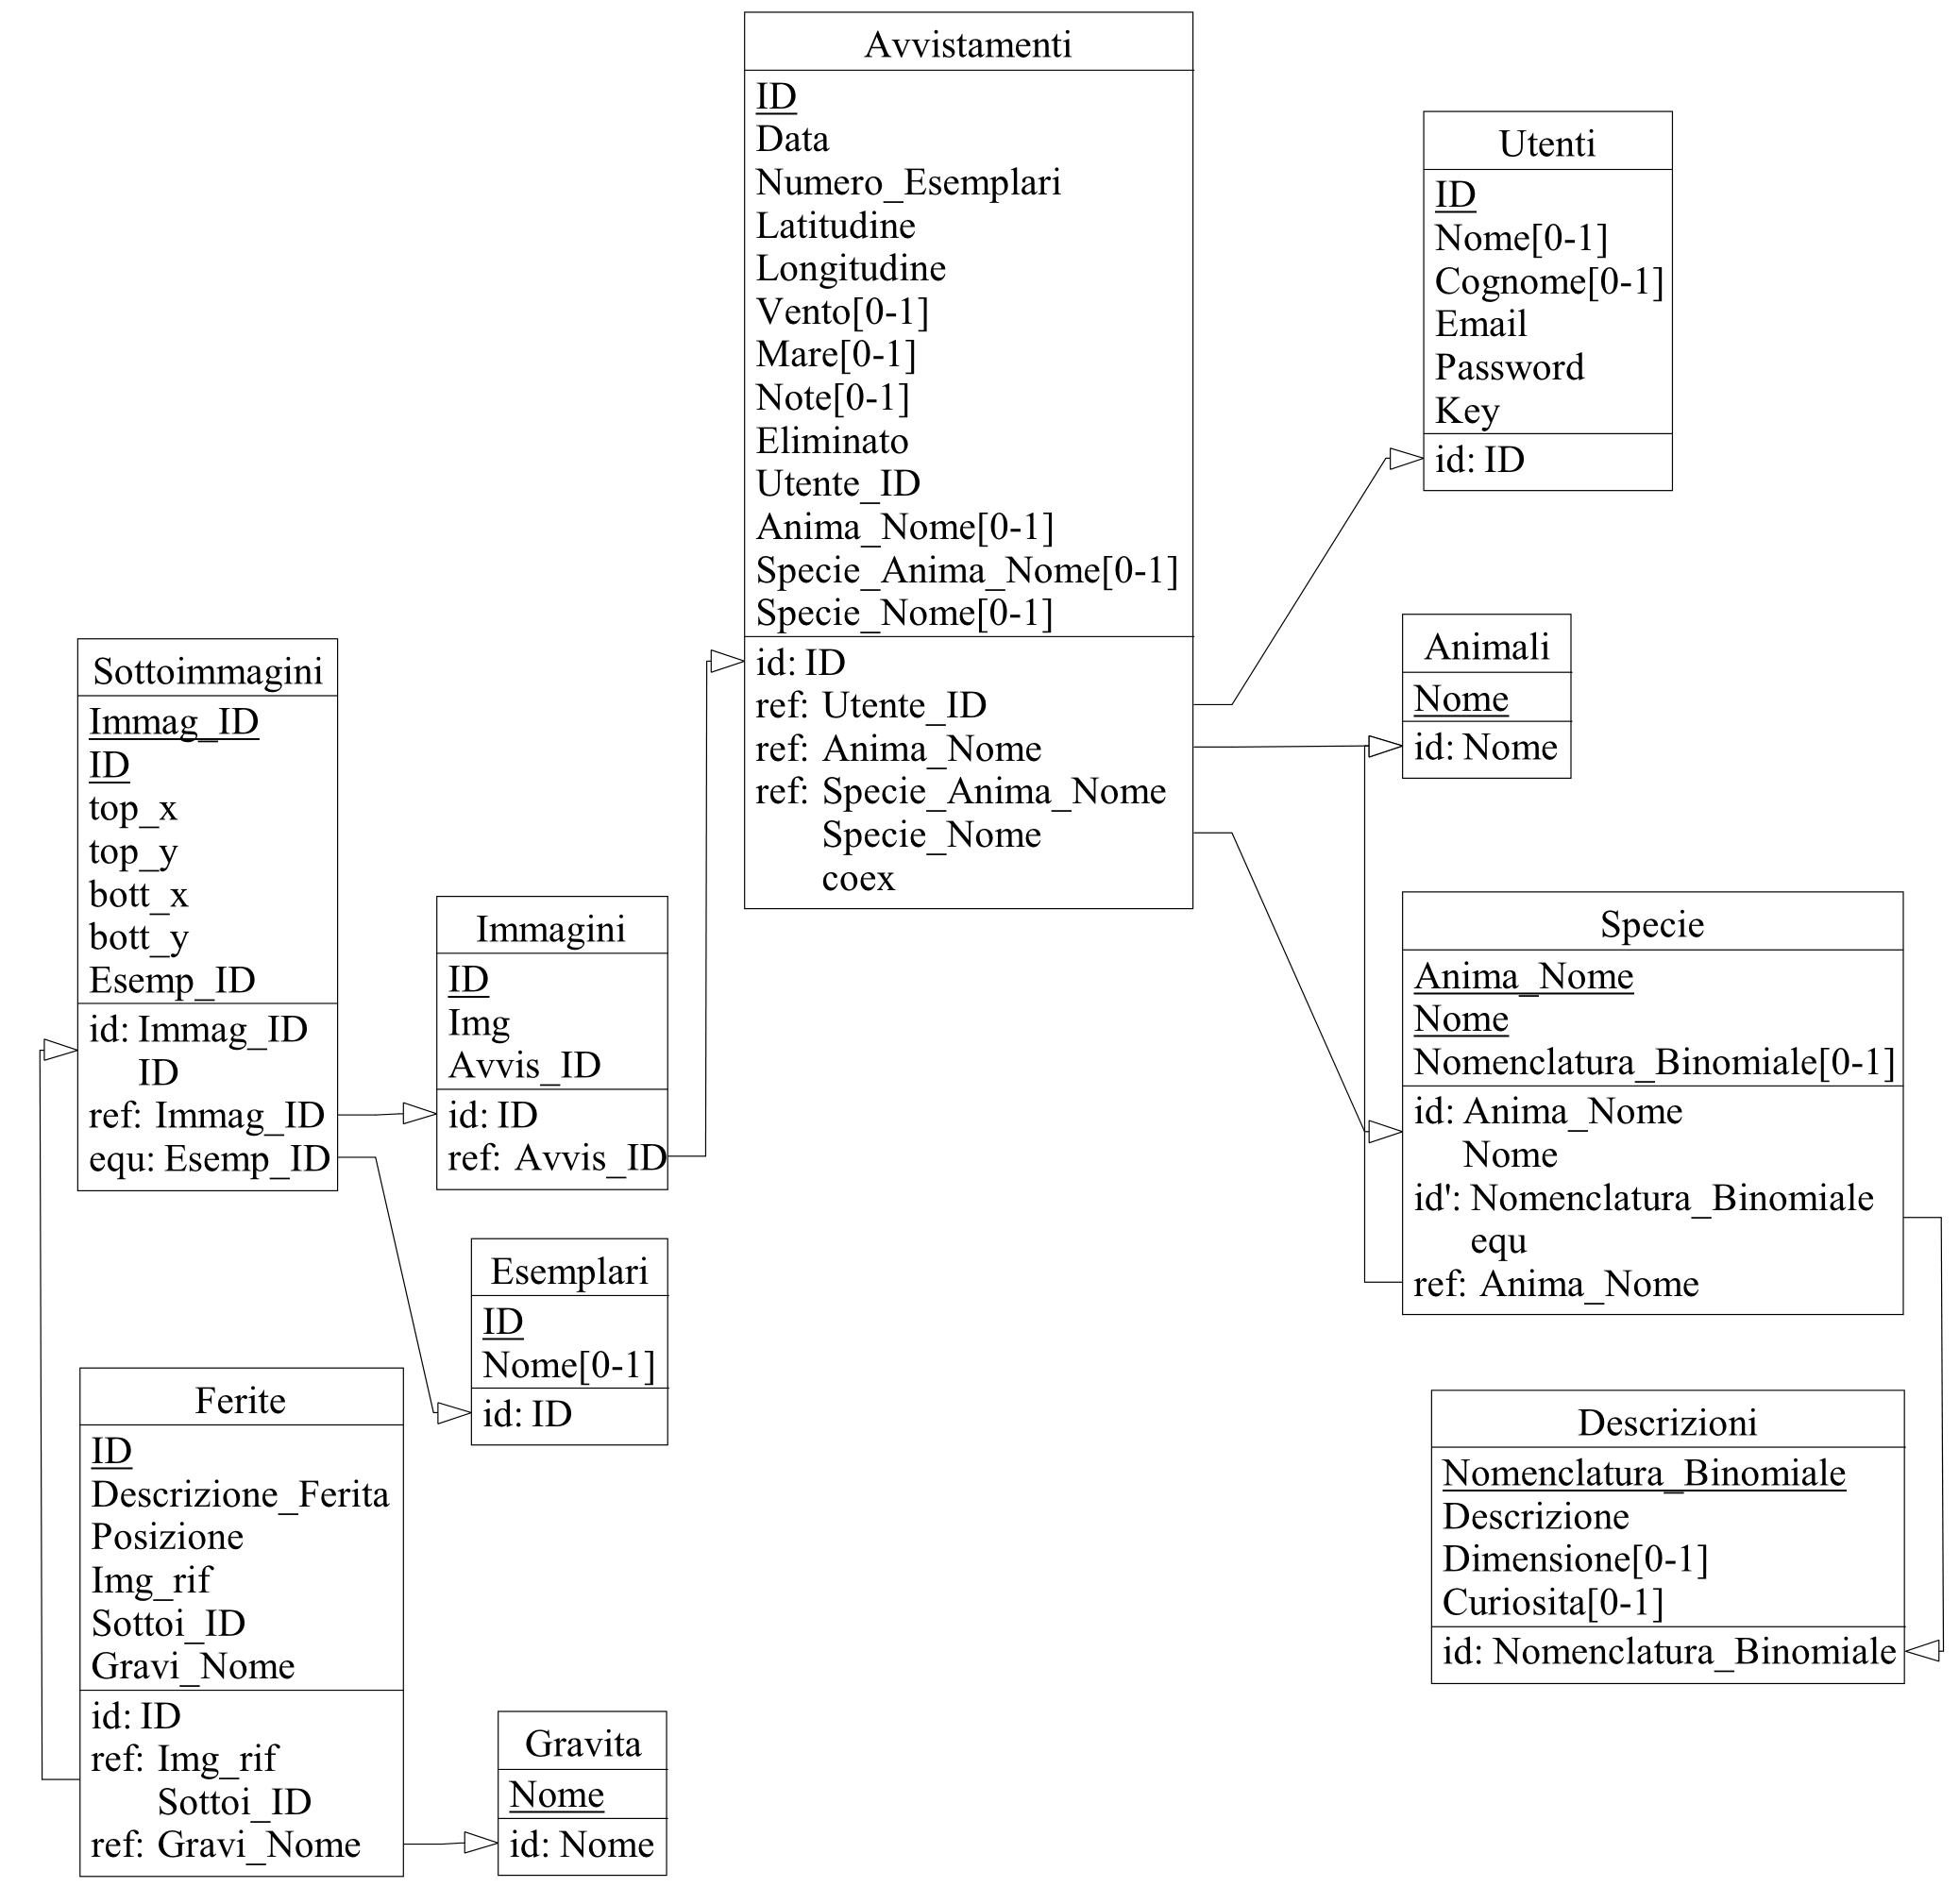
\includegraphics[scale=0.22]{img_concettuale/Logico.png}
\caption{Schema logico finale.}
\end{figure}

\chapter{Documentazione Applicazione Mobile}

\chapter{Documentazione Interfaccia Web}

\section{Progettazione}
Nella progettazione sia dell'applicativo web che mobile si è cercato di dare particolare attenzione alla comunicazione visiva della GUI, nello specifico si è cercato di rispettare i seguenti principi:
\begin{itemize}
\item \textbf{Affordance:} enfatizzare aspetti di un oggetto che invitano a manipolarlo in un certo modo.\\ Tali aspetti possono essere: Tridimensionalità, ombreggiatura e puntamento.
\item \textbf{Metafora:} una parola, una frase o una figura la quale dipinge un oggetto o un concetto attraverso una somiglianza con un altro oggetto del mondo reale. Un esempio è: un bottone rappresenta un comando.
\item \textbf{Layout:} 
la posizione degli elementi all'interno della pagina è uno strumento importante di comunicazione.
\item \textbf{Colori:} utili per focalizzare l'attenzione o suscitare emozioni.
\item \textbf{Font:} leggibilità in relazione al tipo e alle caratteristiche del carattere.
\end{itemize}

\subsection{Usabilità}
Col termine usabilità si intende l'efficacia, l'efficienza e la soddisfazione con cui determinati utenti eseguono determinati compiti in particolari ambienti. 
Più nello specifico in questo applicativo tali termini rappresentano:
\begin{itemize}
\item \textbf{Efficacia:} tutti i compiti richiesti in fasi di analisi possono essere eseguiti senza problematiche.
\item \textbf{Efficienza:} si è cercato di usare al meglio le risorse disponibili per svolgere i compiti richiesti.
\item \textbf{Soddisfazione:} si è avuta prova dell'accettabilità del funzionamento da parte dell'utente.
\end{itemize}

\subsubsection{Personas e scenarios}
Sono state definite delle personas, cioè persone che rappresentano dei gruppi di utenti, i quali saranno gli utilizzatori del programma ed a ognuno di loro è stato associato uno scenario, il quale rappresenta le operazioni, il modo di muoversi nel sito e le modalità di utilizzo di ciascuno di loro.
Le personas che sono state riscontrate:
\begin{itemize}
 \item Responsabile avvistamenti: persona addetta alla modifica delle informazioni al fine di modificare, aggiungere o eliminare i dati. 
\item Ricercatore: persona che carica nuove informazioni, di un nuovo avvistamento direttamente dal portale.
 \end{itemize} 
 A ciascuna di esse è associato uno scenarios:
 \begin{itemize}
 \item Responsabile avvistamenti: iscrizione al sito con possibilità di modifica degli avvistamenti, aggiunta e cancellazione.
 \item Ricercatore: Aggiunta di nuovi avvistamenti.
 \end{itemize}

\subsection{Design}
In questa sezione viene descritto il processo che ha portato alla creazione dell'interfaccia web.
Al fine di progettare la migliore interfaccia con le rispettive caratteristiche che sono stato elencate in fase di analisi sono stati fatti:
\begin{itemize}
\item Focus Group: è stato chiesto agli utilizzatori del sistema come prevedevano la realizzazione di determinate parti di interfaccia, in particolare per le schede dei singoli avvistamenti sono state proposte diverse modalità disposizione dei contenuti e sulla base di un sondaggio è stata scelta la migliore strategia.
\item Mockup: sulla base delle informazioni sono stati creati degli schemi base in cui danno un'idea della struttura del sistema.
\item Experience Prototyping: E' stata realizzata un semplice prototipo di tipo usa e getta al fine di verificare alcune parti incerte del programma in particolare la tabella degli avvistamenti e le specifiche di ogni avvistamento.
\end{itemize}
Gli obiettivi del design sono principalmente di essere:
\begin{itemize}
\item Mobile First
\item User Centered
\item Accessibile
\end{itemize}

\subsubsection{Mockup}
Prima dell'inizio della realizzazione sono stati creati i mockup principali al fine definire la struttura delle pagine. In particolare sono stati creati i mockup per la pagina principale in cui vengono visualizzati tutti i gli avvistamenti e la pagina del singolo avvistamento in cui si definiscono le operazioni chiave.
Il primo mockup che viene mostrato è quello della pagina principale in modalità mobile:
\begin{figure}[hbtp]
\centering
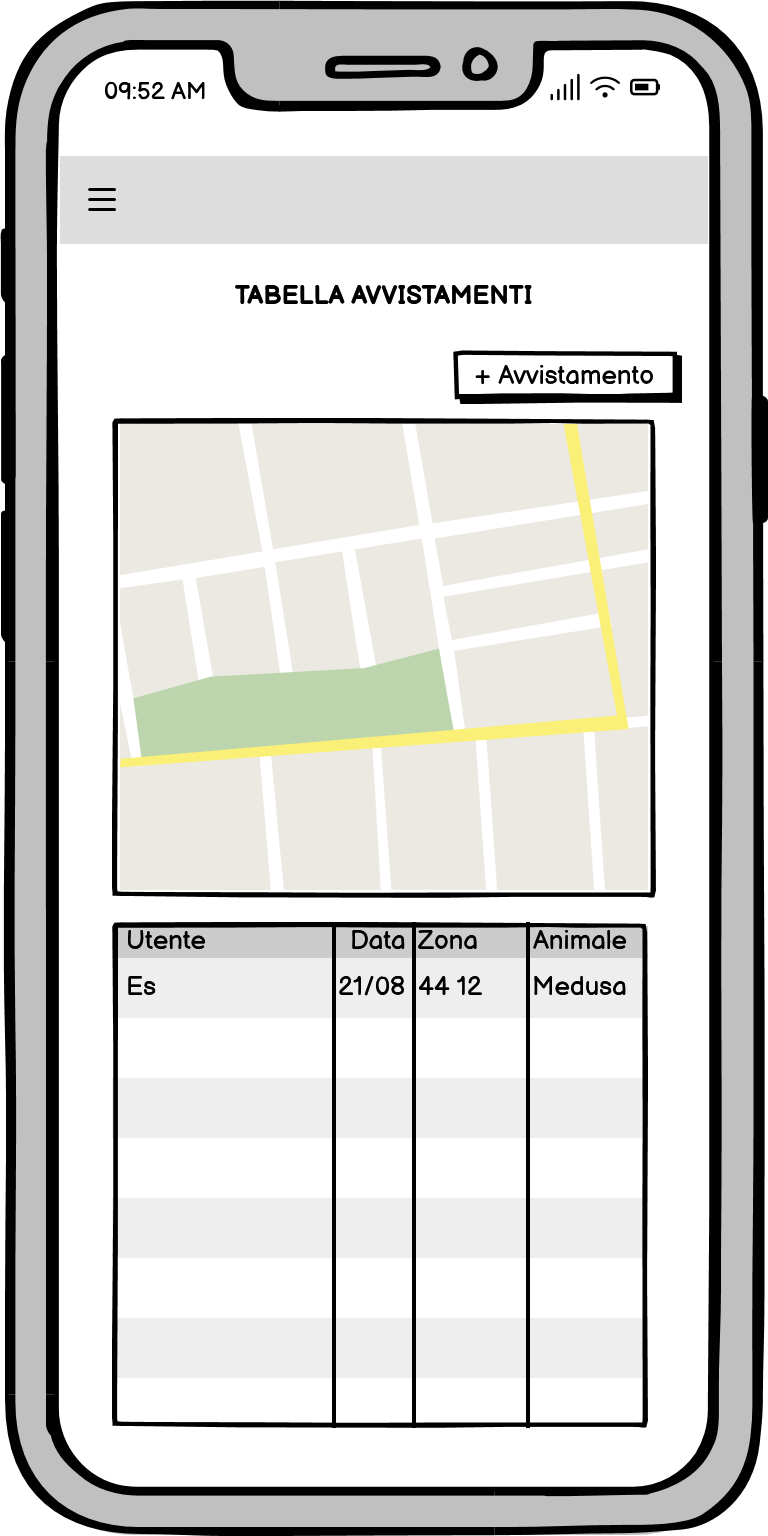
\includegraphics[scale=0.43]{img_concettuale/HomeMob.png}
\caption{Mockup homepage del sito in versione mobile.}
\end{figure}
\\Da come si può vedere dell'immagine, si tratta di un design molto semplice in cui è presente un menù, una mappa e una tabella in cui saranno elencati gli avvistamenti che sono caricati attraverso l'apposito pulsante oppure attraverso l'applicazione mobile.\\
Nel secondo mockup viene mostrata stessa pagina web in versione desktop: 
\begin{figure}[hbtp]
\centering
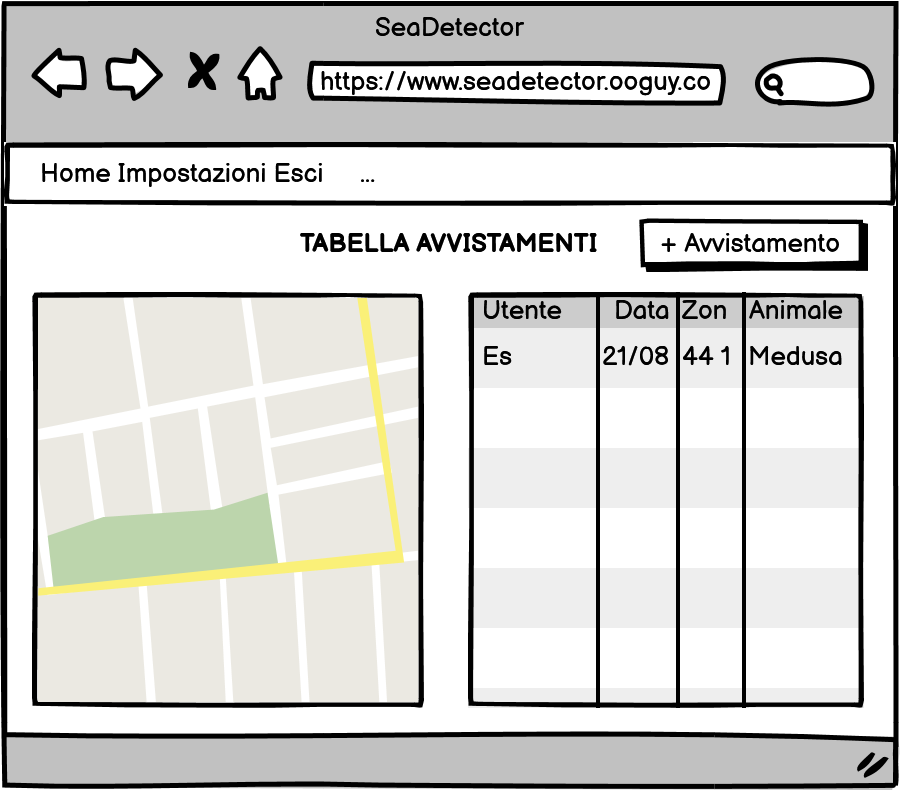
\includegraphics[scale=0.90]{img_concettuale/Home.png}
\caption{Mockup homepage del sito in versione desktop.}
\end{figure}
\\La pagina web contiene gli stessi elementi descritti nell'immagine precedente ma disposti solo in modo differente al fine di adattare lo spazio.
Nel terzo mockup invece viene rappresentata la struttura della pagina degli avvistamenti in versione mobile:
\begin{figure}[hbtp]
\centering
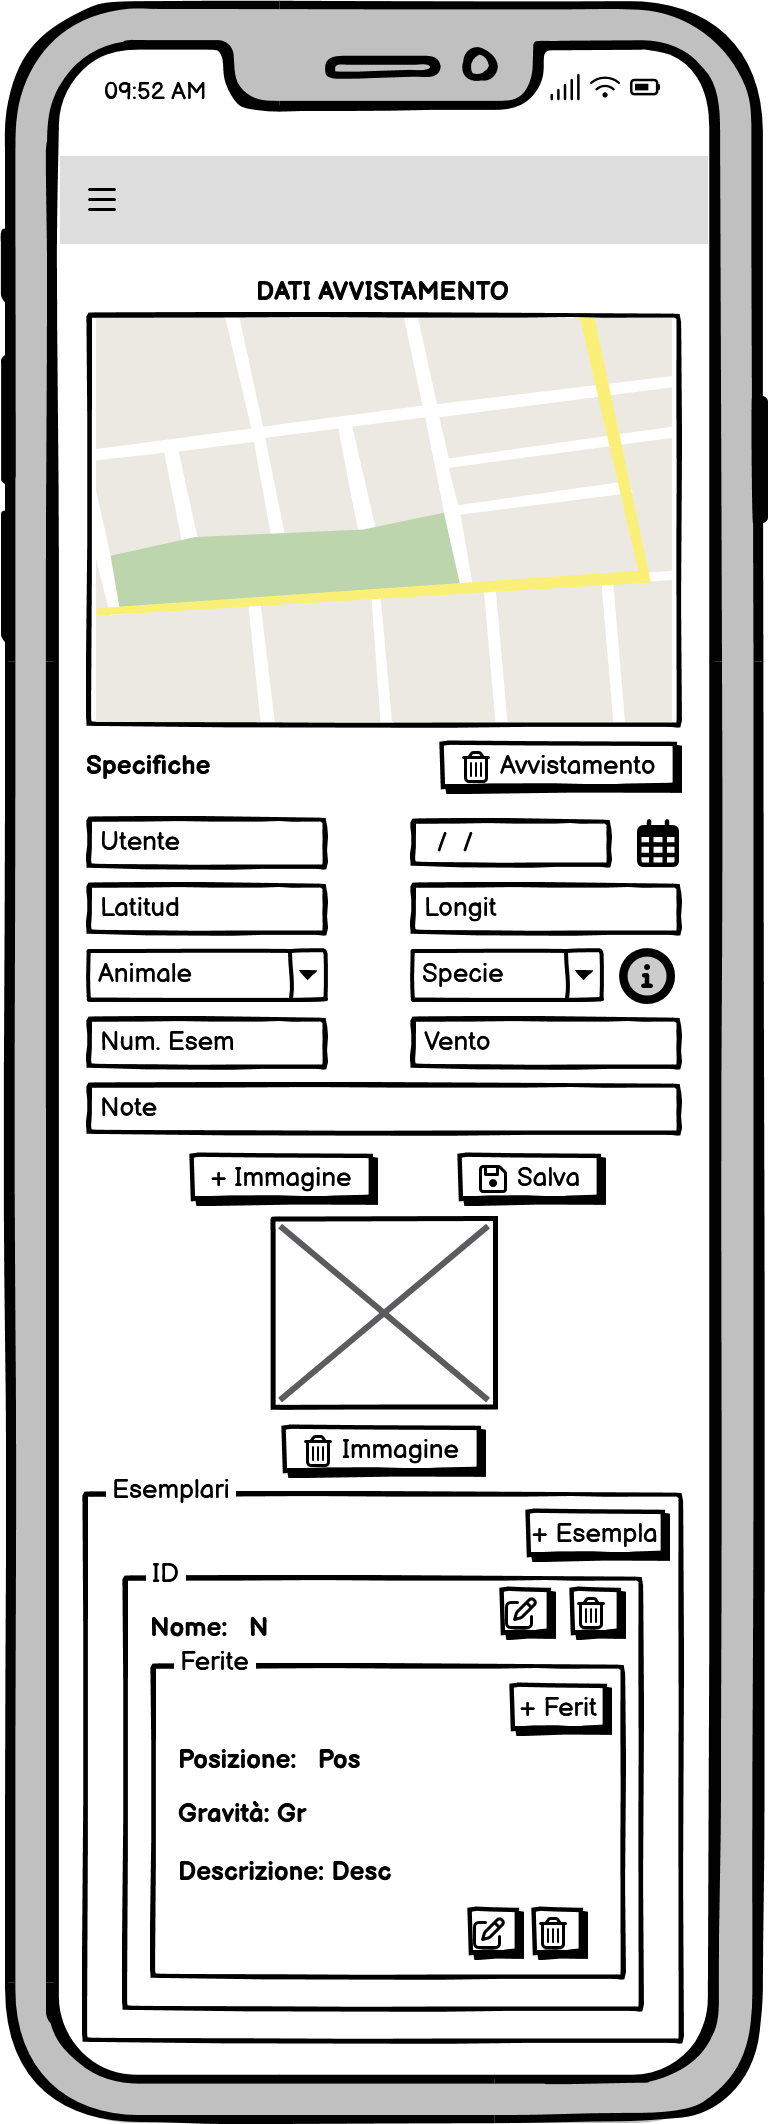
\includegraphics[scale=0.50]{img_concettuale/avvistamentoMok.png}
\caption{Mockup avvistamento del sito in versione mobile.}
\end{figure}
\\La pagina web contiene una semplice mappa in cui viene raffigurato il luogo dell'avvistamento, per ogni avvistamento vengono mostrati i dati, i quali sono modificabili al fine di variare le informazioni precedentemente inserite. In aggiunta per ogni avvistamento c'è la possibilità di aggiungere immagini e di cancellarle. Per ogni immagine possono essere aggiunte più sottoimmagini ognuna delle quali rappresenta un individuo al quale possono essere aggiunte o eliminare le ferite.\\
Nel quarto ed ultimo mockup viene raffigurata la struttura della pagina degli avvistamenti:
\begin{figure}[hbtp]
\centering
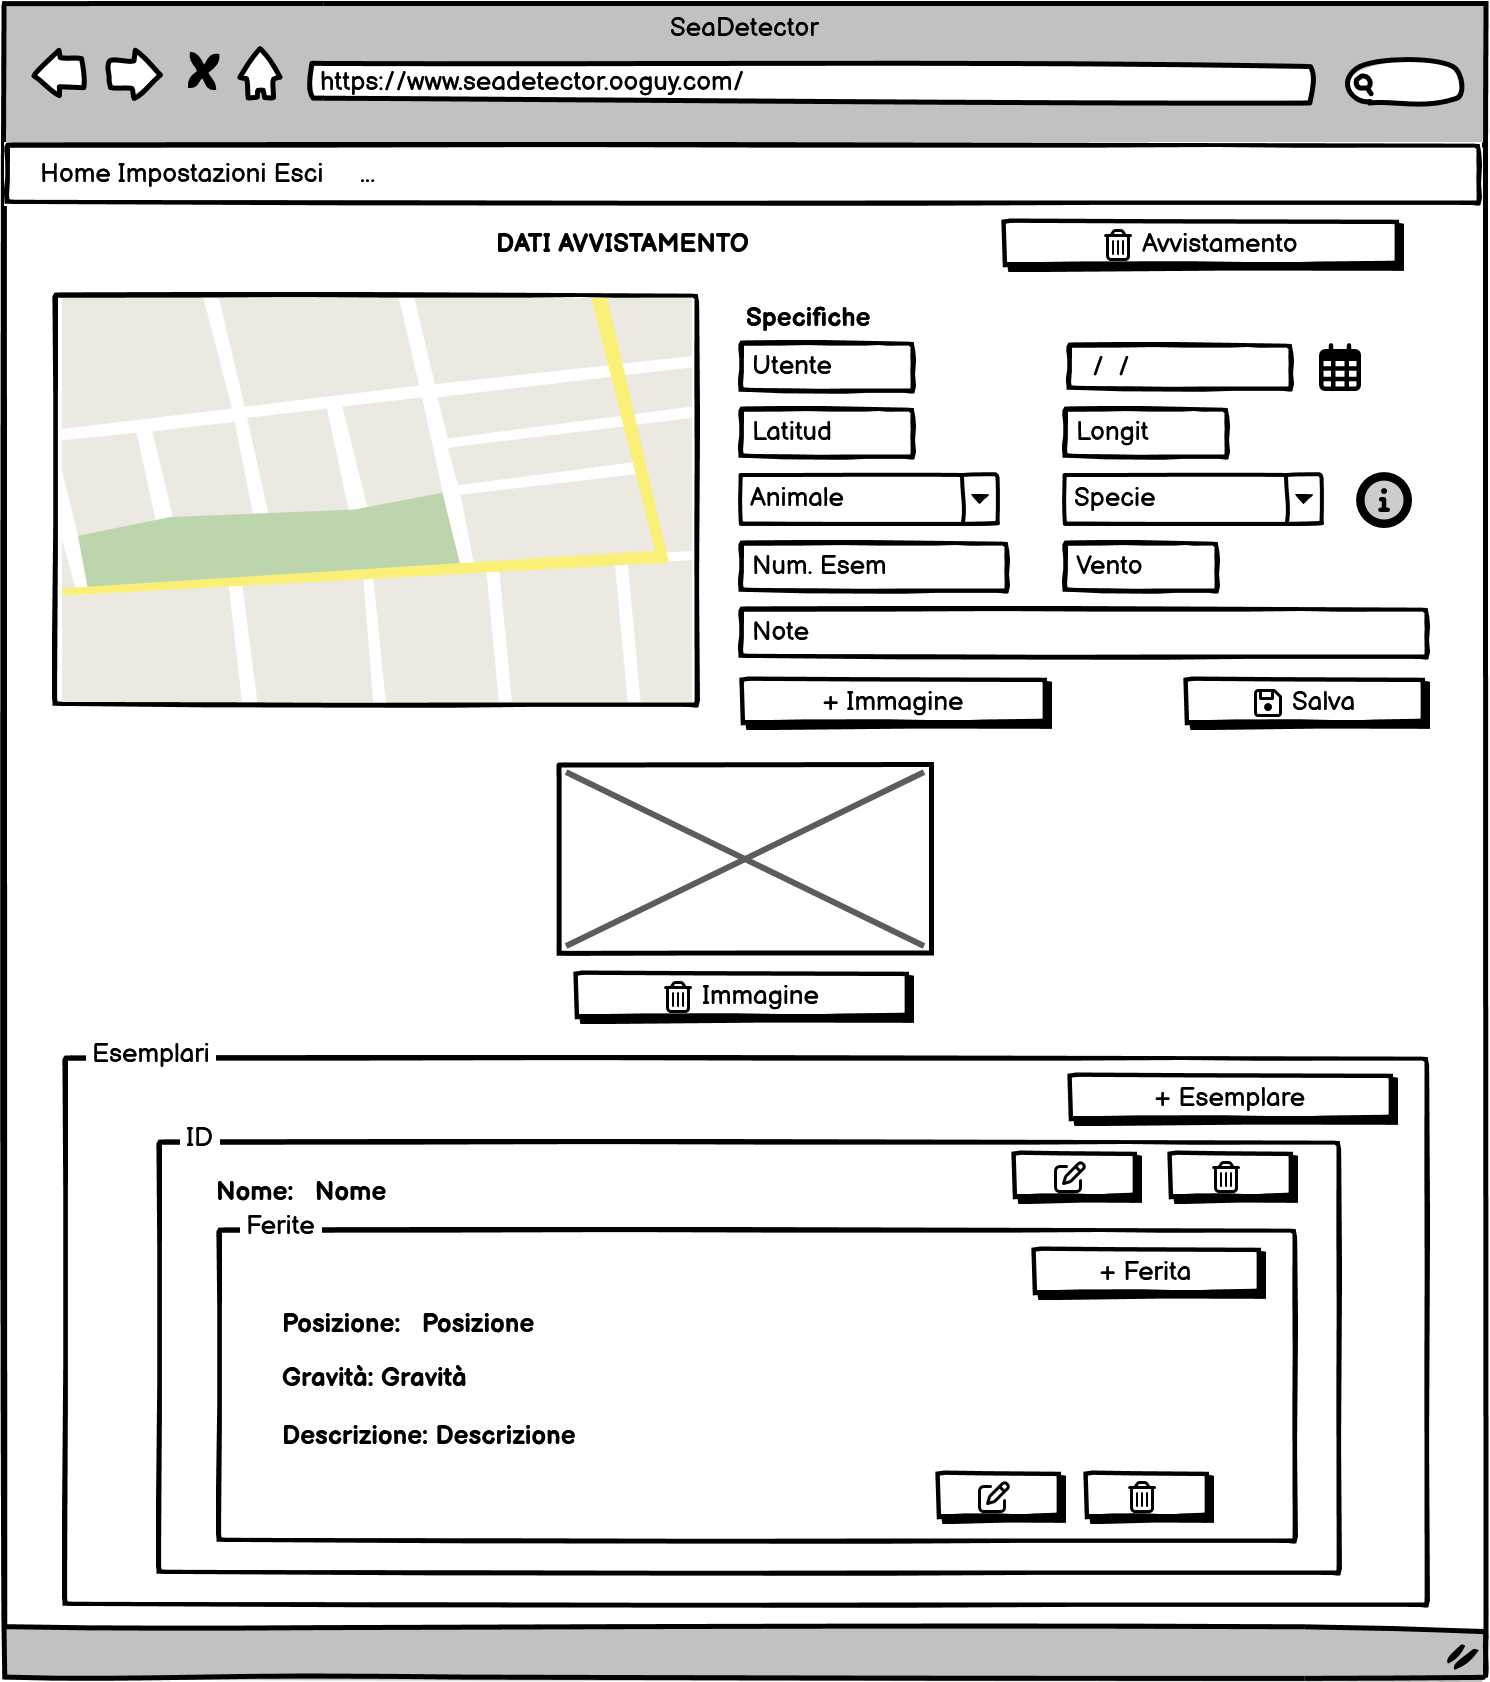
\includegraphics[scale=0.47]{img_concettuale/avvistamentoDesk.png}
\caption{Mockup avvistamento del sito in versione desktop.}
\end{figure}
\\Il contenuto della pagina è lo stesso della versione mobile solo con una disposizione diversa degli elementi.


\subsection{Solution stack}
Un solution stack è un insieme di tecnologie software che vengono utilizzate per costruire un'applicazione o un sistema. È composto da una combinazione di software di sviluppo, linguaggi di programmazione, framework, database e altri strumenti necessari per creare un'applicazione completa e funzionante.
Un solution stack ben sviluppato può rendere molto più semplice e veloce lo sviluppo di un'applicazione, poiché fornisce tutti gli strumenti necessari in un pacchetto completo.\\ 
Esistono molti solution stack differenti disponibili, alcuni dei quali sono sviluppati per specifici sistemi operativi o piattaforme, mentre altri sono più generici e possono essere utilizzati su molte piattaforme diverse.\\

\subsubsection{LAMP}
Nel nostro caso è stato utilizzato il solution stack denominato LAMP (Linux, Apache, MySQL, PHP) è un popolare solution stack per lo sviluppo di applicazioni web su sistemi operativi Linux. Questo perchè il database il server web Apache2 sono situati in una raspberry4 la quale ha un indirizzo di rete fisso al quale chiunque collegato via internet può collegarsi ed accedere al sito e ai suoi contenuti previa registrazione.
\begin{figure}[hbtp]
\centering
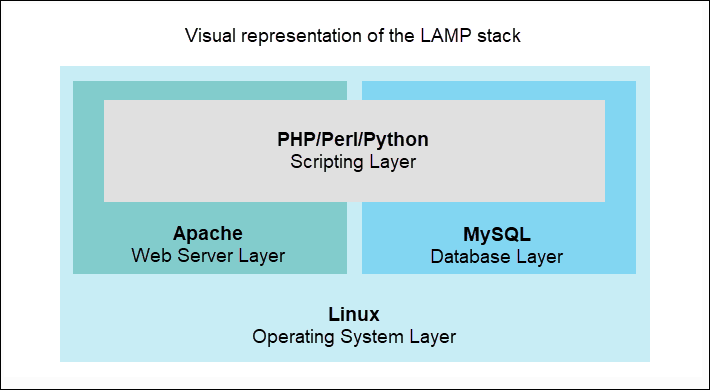
\includegraphics[scale=0.47]{img_concettuale/LAMP.png}
\caption{Stack LAMP}
\end{figure} 
\subsubsection{PHP}
Lato server si ha un linguaggio di programmazione denominato PHP esso è open-source, utilizzato per lo sviluppo di siti web dinamici e interattivi. \\ PHP è un linguaggio di scripting server-side, il che significa che il codice PHP viene eseguito sul server, non sul browser del client. Questo rende il processo di sviluppo più efficiente, poiché l'elaborazione avviene sul server e i dati vengono inviati al browser solo una volta elaborati. Questo rende possibile creare siti web dinamici e interattivi, che possono essere personalizzati in base alle esigenze dell'utente. \\ Esso supporta anche molte funzionalità avanzate, come l'elaborazione di form HTML, la connessione a database, l'elaborazione di cookie e sessioni, e la gestione dei file. Questo rende possibile creare siti web dinamici che possono offrire molte funzionalità avanzate, come ad esempio la personalizzazione dei contenuti in base alle preferenze dell'utente.

\subsubsection{MYSQL}
MySQL è un sistema di gestione del database relazionale open-source, utilizzato per gestire grandi quantità di informazioni. Il fatto che sia un sistema di gestione del database relazionale, significa che i dati sono organizzati in tabelle e ogni tabella ha una relazione con le altre. Questo rende il processo di gestione dei dati molto efficiente e semplice, poiché è possibile accedere rapidamente a informazioni specifiche utilizzando delle query. Esso è un sistema di gestione del database altamente scalabile, il che significa che può gestire grandi quantità di informazioni senza compromettere le prestazioni. Inoltre, è molto flessibile e facile da usare, il che significa che gli sviluppatori possono facilmente creare e gestire grandi quantità di informazioni.

\subsection{Fruizione del servizio}
Il servizio essendo di tipo centralizzato su un unico server è fruibile utilizzando le tre tecnologie che sono alla base del web.
\begin{figure}[hbtp]
\centering
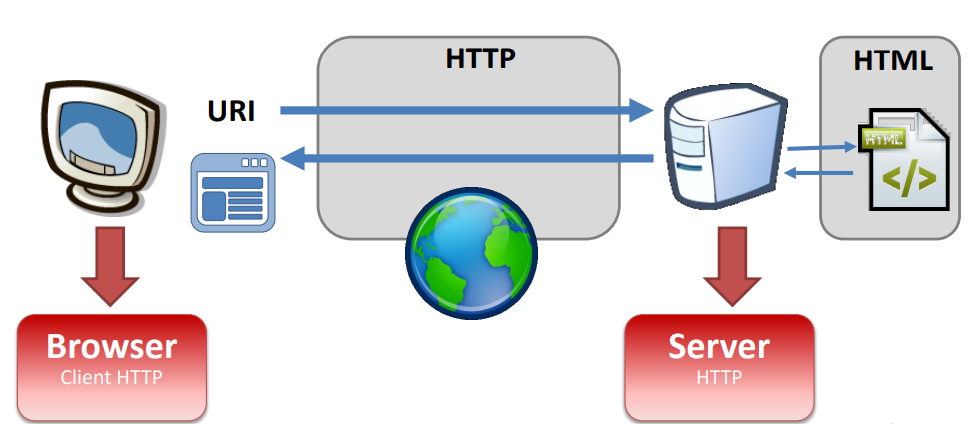
\includegraphics[scale=0.60]{img_concettuale/tecnologie.png}
\caption{Tecnologie alla base del web}
\end{figure} 

\subsubsection{URI}
Lo Uniform Resource Identifier è utilizzato per identificare risorse in modo univoco e permanente. Questo è importante perché rende possibile accedere alle risorse su Internet in modo affidabile e coerente, indipendentemente dalla loro posizione. Nel nostro caso si può utilizzare l'URL \textit{www.seadetector.ooguy.com} al fine di raggiungere il sito.

\subsubsection{HTTPS}
L'Hypertext Transfer Protocol Secure è un'estensione di HTTP, il protocollo di base utilizzato per la trasmissione di informazioni su internet. Il funzionamento di HTTPS si basa sulla crittografia. Quando un utente accede a un sito web che utilizza HTTPS, i dati inviati e ricevuti vengono crittografati utilizzando un certificato SSL (Secure Sockets Layer) o TLS (Transport Layer Security). Questo certificato garantisce che i dati siano protetti da eventuali attacchi esterni e che solo l'utente e il sito web abbiano accesso ai dati scambiati.
L'utilizzo di HTTPS è molto importante per la sicurezza delle informazioni personali e sensibili degli utenti. Ad esempio, quando si effettua un login i dati sensibili come le password vengono trasmessi attraverso internet. Se il sito web utilizza HTTPS, questi dati vengono protetti da eventuali attacchi esterni e non possono essere intercettati o utilizzati impropriamente.\\
In particolare nel nostro caso una volta installato e configurato il server web sulla Ruspberry pi4 è stato utilizzato un software denominato certbot il quale facilita la creazione, l'installazione e l'utilizzo di certificati SSL per i siti web. Inoltre, Certbot si occupa automaticamente della gestione dei certificati, inclusa la rinnovazione automatica dei certificati prima della loro scadenza. Questo rende molto più semplice la gestione dei certificati SSL, poiché gli sviluppatori non devono preoccuparsi di rinnovare manualmente i certificati.\\
Certbot permette di ottenere certificati gratuiti tramite Let's Encrypt, un'organizzazione che fornisce certificati SSL gratuiti a tutti.\\

\subsubsection{HTML}
Quindi una volta contattato il server attraverso l'identificatore e utilizzando il protocollo di file transfert in modalità sicura il client e il server si scambiano le pagine in formato HTML.\\
HTML (Hypertext Markup Language) è un linguaggio di markup utilizzato per creare documenti web. HTML definisce la struttura e il contenuto della pagina web, utilizzando un insieme di tag per identificare diversi elementi della pagina, come il testo, le immagini, i link e molto altro.

\subsection{Stile}
Per quanto riguarda lo stile del sito sono state utilizzate diverse tecnologie combinate insieme per cercare di avere la massima resa possibile.

\subsubsection{CSS}
CSS (Cascading Style Sheets) è un linguaggio di marcatura utilizzato per descrivere l'aspetto di un documento HTML. Esso è un componente importante della creazione di siti web, poiché permette ai designer e agli sviluppatori di separare il contenuto di una pagina web dalla sua presentazione. In questo modo il contenuto di una pagina web può essere modificato senza influire sulla sua presentazione, rendendo più semplice la manutenzione e l'aggiornamento del sito. CSS viene utilizzato per la creazione di layout complessi, animazioni, transizioni e effetti grafici. 

\subsubsection{Bootstrap}
Bootstrap è un framework di design per il web, che fornisce un insieme di componenti e strumenti per la creazione di siti web. Bootstrap è progettato per aiutare i designer e gli sviluppatori a creare progetti web più velocemente e con maggiore facilità, fornendo una serie di componenti predefiniti e stili per la creazione di interfacce utente. Bootstrap è basato su HTML, CSS e JavaScript, e offre una vasta gamma di componenti, tra cui barre di navigazione, moduli, tabelle, pulsanti, icone, griglie e molto altro.
Esso rende molto più semplice la creazione di progetti web, invece di dover scrivere da zero il codice CSS e HTML per ogni progetto, i designer e gli sviluppatori possono utilizzare i componenti predefiniti di Bootstrap, che sono già ben testati e ottimizzati per una buona esperienza utente.
Un altro spetto fondamentale è che esso è basato sul principio denominato Mobile first e questo permette di creare pagine web adatte oltre che per pc anche per cellulari. Grazie alla combinazione di righe e colonne che insieme formano una griglia, permettono di modificare il layout della pagina in base alla grandezza del dispositivo che si utilizza.

\subsection{Javascript e Librerire}
Per l'applicazione è stato usato Javascript come linguaggio di programmazione lato client esso è dinamico e interpretato, utilizzato principalmente per creare interazioni ed effetti visivi sulle pagine web. Esso è un linguaggio di programmazione completamente differente rispetto a HTML e CSS, che sono utilizzati per la creazione della struttura e del design delle pagine web. JavaScript, d'altra parte, è utilizzato per creare interazioni e effetti dinamici all'interno della pagina, come ad esempio la validazione dei moduli e la creazione di animazioni.
\subsubsection{JQUERY}
Nel progetto al fine di semplificare la crezione di determinate funzionalità è stato utilizzata una libreria JavaScript open source utilizzata per rendere più semplice e veloce lo sviluppo di pagine web interattive e applicazioni web. Essa è denominata JQUERY la sua principale caratteristica è la sua capacità di semplificare le attività di sviluppo web, come la manipolazione del DOM (Document Object Model), l'aggiunta di effetti e animazioni e la gestione degli eventi. Essa ha la caratteristica di essere molto compatibile con i browser più diffusi e offre un'ottima compatibilità anche con i dispositivi mobile.
\subsubsection{AJAX}
\begin{figure}[hbtp]
\centering
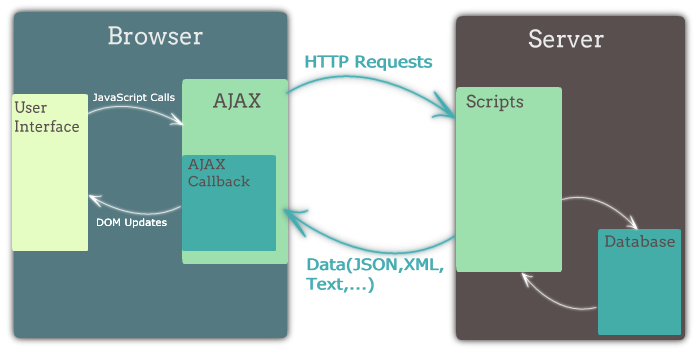
\includegraphics[scale=0.45]{img_concettuale/ajax.jpg}
\caption{Funzionamento di AJAX}
\end{figure} 
Nell'applicazione per richiedere dati dal database vengono eseguite delle chiamate Ajax asincrone al server. AJAX (Asynchronous JavaScript and XML) è una tecnologia utilizzata per creare applicazioni web dinamiche e interattive. Esso si basa sull'utilizzo di JavaScript e permette di aggiornare parti di una pagina web senza dover ricaricare l'intera pagina.
Invece di inviare una richiesta al server per ottenere l'intera pagina web, AJAX consente di inviare richieste al server per ottenere solo i dati necessari. Questo significa che, ad esempio, se un utente clicca su un link o modifica una form, solo i dati necessari vengono inviati al server, e solo la parte della pagina che deve essere aggiornata viene effettivamente modificata. Questo rende l'interazione più veloce e fluida per l'utente, poiché non è necessario attendere il caricamento dell'intera pagina ogni volta che viene effettuata un'azione.
Il server invierà i dati richiesti dal client in formato JSON.

\subsubsection{PHPMailer}
Nel sito al fine di recuperare la password nel caso qualcuno se la dimentichi in fase di login è stata implementata una funzione che permetta di inviare email con all'interno la password temporanea dell'account. Per farlo è stata utilizzata la libreria PHP Mailer. Essa è una libreria open-source per PHP che permette di inviare email tramite il protocollo SMTP (Simple Mail Transfer Protocol). Questa libreria è stata sviluppata per semplificare il processo di invio di email da un sito web, e offre molte funzionalità avanzate, come ad esempio la gestione della codifica dei caratteri e l'invio di email con allegati. La libreria PHPMailer è molto semplice da utilizzare e offre un'interfaccia intuitiva per l'invio di email da un sito web.\\
AL fine di non dover comprare un dominio per le mail e dover gestire il server mail è stato utilizzato il servizio di posta elettronica di Libero.

\subsection{Cookies}
Esistono diverse tecniche utilizzate per raccogliere i dati online e costituire, attraverso esse, un profilo dell'utente. Una di queste tecniche prevede l'utilizzo di cookies, essi sono considerati delle stringhe di testo che il browser crea all'apertura di una pagina web sul computer dell'utente e che salvano dati dell'utente durante la navigazione di un sito web agevolandone l'utilizzo. Dei possibili esempi possono essere:
\begin{itemize}
\item Memorizzare le preferenze linguistiche.
\item I dati di login.
\end{itemize}
I dati vengono memorizzati per essere poi ritrasmessi ai medesimi siti alla visita successiva dello stesso utente. Mediante i cookies è anche possibile monitorare la navigazione e raccogliere dati inerenti alle abitudini e le scelte personali degli utenti, consentendo così la creazione di profili dettagliati degli utenti. Un esempio è la personalizzazione delle inserzioni pubblicitarie sul browser. Generalmente un cookie contiene un attributo che indica la durata di vita e un numero generato in modo casuale che consente il riconoscimento dell'utente.\\
Esiste una specifica normativa, di derivazione europea, che disciplina l'utilizzo dei cookies al fine di tutelare le persone da forme di profilazione definite occulte e di consentirgli
un minimo controllo sulla circolazione dei dati inerenti alla propria navigazione online.\\
Esistono tre tipologie di cookies:
\begin{enumerate}
\item \textbf{Cookies tecnici:} necessari per motivi tecnici e comportano una forma indispensabile (e molte volte temporanea) di memorizzazione di dati. Essi consentono la normale navigazione di un sito o la implementazione di un servizio, salvando solo le preferenze ed i criteri di navigazione di ogni utente.
\item \textbf{Cookies di profilazione:} elementi che non sono tecnicamente necessari per il funzionamento del sito. Alcuni esempi sono i cookies di tracciamento, oppure ai cookies che creano profili dell'utente per finalità pubblicitarie e vengono utilizzati per finalità di marketing.
\item \textbf{Cookies analitici:} consentono il monitoraggio dell'uso del sito da parte degli utenti e consentono il miglioramento del sito stesso. Talvolta anche i cookies analitici possono essere di terze parti.
\end{enumerate}
Nel nostro applicativo sono stati utilizzati solo cookies tecnici, al fine di memorizzare i dati di login. Quindi secondo la normativa, i cookies tecnici possono essere usati anche senza chiedere il consenso dell'utente. Al fine dell'applicazione si è deciso di non utilizzare cookies di profilazione e nemmeno quelli analitici.

\subsection{Sicurezza}
Oltre all'utilizzo di un protocollo https si è data una particolare attenzione alla sicurezza sia per quanto riguarda la trasmissione dei dati tecnici degli avvistamenti che quelli personali come ad esempio le password.
\subsubsection{Invio dati} 
Tutte le form, chiamate ajax inviano i dati in modalità POST. Il metodo "POST" è una delle due modalità principali per inviare dati tramite una richiesta HTTP. Quando si inviano dati utilizzando il metodo POST, i dati sono inclusi nella corpo della richiesta HTTP, anziché nell'URL come con il metodo GET. Questo rende il metodo POST adatto per l'invio di dati sensibili o confidenziali, poiché i dati non sono visibili nell'URL e non possono essere facilmente intercettati o modificati.

\subsubsection{Criptaggio password} 
Per quanto riguarda la password si è usata una tecnica leggermente complicata:
\begin{figure}[hbtp]
\centering
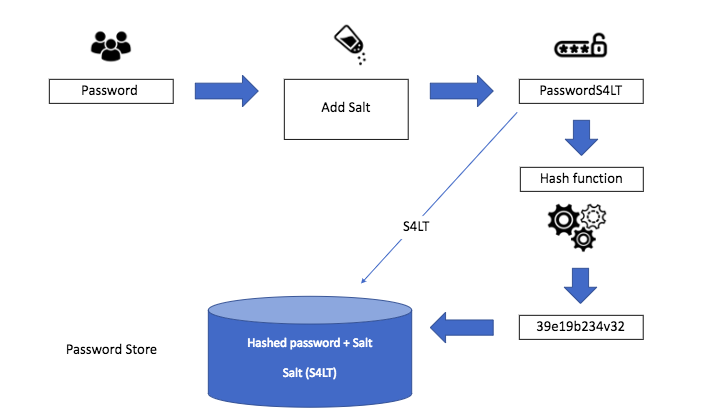
\includegraphics[scale=0.42]{img_concettuale/sale.png}
\caption{Struttura alla base della fase di criptaggio}
\end{figure}
 
\begin{enumerate}
\item In fase di registrazione l'utente inserisce due volte la password in modo da evitare errori di battitura.
\item Quando conferma i dati inseriti viene creata una chiave univoca basata sul timestamp del momento e criptata utilizzando una funzione hash SHA1 (SALT).
\item Una volta calcolata la chiave criptata viene utilizzata come chiave di codifica per cifrare la password inserita dell'utente attraverso l'algoritmo di crittografia a chiave simmetrica denominato HMACSHA512. 
\item Avendo la password e la chiave entrambe criptate, oltre a tutti gli altri dati, verrà salvato tutto nel database.
\item Una volta che l'utente esegue l'accesso, il client richiederà al server la chiave al fine di criptare la password e la invierà al server, a questo punto il server confronterà le due password in caso di uguaglianza permetterà l'accesso al servizio.
\end{enumerate}
In questo modo la password dell'utente per l'accesso al sistema non verrà mai trasmessa in rete permettendo maggiore sicurezza in caso di attacchi di tipo Sniffing, man in the middle, o Spoofing.  

\section{Accessibilità}
L'accessibilità informatica è la capacità per i sistemi informatici di fornire servizi e informazioni utilizzabili senza discriminazioni per tutti, compresi coloro che hanno bisogno di tecnologie assistive o configurazioni speciali a causa di disabilità. Questo viene realizzato nei limiti delle attuali conoscenze tecnologiche. Per quanto riguarda il sito si sono prese in considerazione i seguenti tipi di disabilità:
\begin{itemize}
\item Visive
\begin{itemize}
\item Daltonismo
\item Ipovisione (tool assitivi di ingrandimento)
\item Cecità (accesso attraverso screen reader e voice browser)
\end{itemize}
\item Motorie (Utilizzo di strumenti di input diversi)
\end{itemize}

\subsection{WCAG}
L'intero sito internet segue le linee guida create dal W3C per i diversi livelli di accessibilità.
In particolare il WAI è l'acronimo di Web Accessibility Initiative ed è un'iniziativa del W3C. Il cui obiettivo è di promuovere la creazione di contenuti web accessibili e di garantire che tutti gli utenti, indipendentemente dalla loro abilità, possano accedere e interagire con i contenuti del web in modo efficiente e significativo. Il WAI lavora in stretta collaborazione con organizzazioni governative, industriali e di advocacy per garantire che le linee guida e le tecnologie sviluppate siano adatte alle esigenze di tutti gli utenti del web. Il suo impegno a supportare l'accessibilità del web ha contribuito a rendere il web un luogo più inclusivo e accessibile per tutti gli utenti.\\
Le linee guida prese in considerazione sono le WCAG che è l'acronimo di Web Content Accessibility Guidelines.
Esse si basano su 4 principi:
\begin{itemize}
\item Percepibile
\item Utilizzabile
\item Comprensibile
\item Robusto
\end{itemize}
Dai 4 principi discendono le 12 linee guida che
forniscono indicazioni per rendere il contenuto più accessibile. per ciascuna di esse sono stati identificati una serie di criteri di successo che possono essere facilmente verificati. Questi criteri sono suddivisi in tre livelli di conformità: A (minimo), AA e AAA (massimo). Il livello A rappresenta il livello minimo di conformità, mentre il livello AAA rappresenta il massimo livello di conformità possibile.

\begin{figure}[hbtp]
\centering
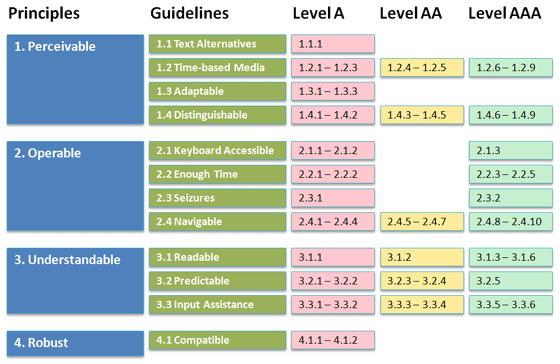
\includegraphics[scale=0.50]{img_concettuale/wcag.png}
\caption{Struttura delle linee guide coi rispettivi livelli.}
\end{figure}

Il WCAG è stato sviluppato con la collaborazione di una vasta comunità di esperti in accessibilità, tecnologia e advocacy e viene continuamente aggiornato per tener conto delle evoluzioni delle tecnologie e delle esigenze degli utenti. Esso è diventato un punto di riferimento per gli sviluppatori di siti web e per le organizzazioni che cercano di garantire l'accessibilità dei loro contenuti web.

\subsubsection{Linee guida}
Nel progetto le linee guida a cui si è data maggiore importanza sono state:\\
\emph{Principio Percettibile:}
\begin{itemize}
\item Linea guida 1.1 Alternative testuali: Si necessita di fornire alternative testuali per qualsiasi contenuto non di testo in modo che
questo possa essere trasformato in altre forme fruibili secondo le necessità degli utenti come Braille, stampa a caratteri ingranditi, sintesi vocale o in un linguaggio più semplice.
\begin{itemize}
\item Criterio di successo 1.1.1; Contenuti non testuali: Tutti i contenuti non testuali presentati all'utente hanno un'alternativa testuale equivalente. Questo viene fatto con l'utilizzo in modo opportuno dei tag figure, figcaption oppure con gli attributi alt oppure longdesc nei tag img.
\end{itemize}
\item Linea guida 1.4 Distinguibile: Rendere più semplice agli utenti la visione dei contenuti, separando i contenuti in primo piano dallo sfondo.
\begin{itemize}
\item Criterio di successo 1.4.3 Contrasto (minimo): La rappresentazione visiva del testo e di immagini contenenti testo ha un rapporto di
contrasto di almeno 4.5:1.
\end{itemize}

\item Linea guida 1.3 Adattabile: Creare contenuti che possano essere rappresentati in modalità differenti (ad esempio, con layout più semplici), senza perdere informazioni o la struttura.
\begin{itemize}
\item Questa linea guida tratta molte componenti che sono fondamentali nella costruzione della struttura di un documento, in particolare gli elementi della categoria Sectioning hanno funzione strutturale. La struttura del documento è importante non solo per supportare la navigazione con l'ausilio di uno screen reader, ma anche per ottimizzare l'indicizzazione da parte dei motori di ricerca (SEO). La struttura del documento permette una navigazione più fluida tra sezioni, titoli e link.
\end{itemize}
In particolare gli screen reader permettono all'utente non vedenti di percorrere la pagine attraverso i tag di heading. Per questo motivo i tag non devono assolutamente avere uno scopo presentazionale ma la loro sequenza deve essere corretta al fine di aiutare gli utenti che utilizzano mezzi assistivi.\\
Un altro aspetto da tenere in considerazione sono le tabelle che sono presenti nel sito web, queste tabelle per essere accessibili devono utilizzare l'attributo id nei tag di heading(th) e l'attributo headers nei tag td al fine di permettere l'associazione di quella cella con il rispettivo titolo. In aggiunta nei tag di intestazione deve essere utilizzato l'attributo scope, esso permette di identificare lo scopo di quella cella. Per finire, al fine di far capire all'utente quali dati tale tabella rappresenta è utile utilizzare il tag caption dove viene scritta la didascalia della tabella.
\end{itemize}
\emph{Principio Percettibile:}
\begin{itemize}
\item – Linea guida 3.3 Assistenza nell'inserimento: Aiutare gli utenti ad evitare gli errori ed agevolarli nella loro correzione. In particolare,  Fornire etichette o istruzioni quando il contenuto richiede azioni di input da parte dell'utente.\\
La soluzione è l'utilizzo di label con attributo for e input con attributo id, oppure inserire il tag input all'interno della label.
\end{itemize}

\section{Struttura delle pagine}



\chapter{Documentazione Algoritmo Di Riconoscimento}

\chapter{Documentazione Test}




\section{Test con l'utente}
Al fine di effettuare operazioni di test direttamente con l'utente di è deciso di creare un prototipo per far interagire direttamente l'utente sull'intero sistema in beta-release.
Gli aspetti testati sono:
\begin{itemize}
\item Il modello concettuale è sufficientemente rappresentato.
\item Rispetto al progetto l'interfaccia è adatta e sono stati rispettati tutti gli standard.
\item Possibilità di uso alternativo tra mouse e tastiera.
\item Livello di interazione tra l'utente e l'interfaccia.
\item Adeguato bilanciamento tra flusso predefinito e flessibilità.
\end{itemize}
\chapter{Conclusioni}

\chapter{Utilità}
Capitolo di elementi da inserire nei capitoli precedenti.



\section{Ingegneria del software}



\subsection{Verifica del software}
Questa fase ha lo scopo di verificare che il sistema contenga le specifiche di progetto. Tale operazione non viene eseguita solo sul prodotto finale ma segue il progetto ad ogni suo passo.\\
Le tecniche di verifica che sono stato utilizzate sono:
\begin{itemize}
\item \textbf{Di testing:} che attraverso delle prove sperimentali, su un insieme rappresentativo di situazioni, verificano il corretto funzionamento del sistema. 
\item \textbf{Di analisi:} attraverso l'analisi della struttura dei moduli e del codice che li realizza viene verificato il corretto funzionamento. 
\end{itemize}

\subsubsection{Testing}
"Le operazioni di testing possono individuare la presenza di errori nel software ma non possono dimostrarne la correttezza."\cite{1}\\
Come primo passo si sono individuati i casi significativi in cui applicare tale processo.\\
Le operazioni di testing si suddividono in:
\begin{enumerate}
\item \textbf{Testing in the small:} Riguardano porzioni specifiche di codice a cui è stata attribuita una particolare importanza.
\item \textbf{Testing in the large:} riguardano tutto il sistema.
\end{enumerate}

Nel primo caso si è cercato di seguire il seguente criterio di copertura:\\
\textbf{Criterio di copertura delle decisioni e delle condizioni:} selezionare un insieme di test T tali che, a seguito dell’esecuzione del programma P su tutti i casi di T, ogni arco del grafo di controllo di P sia attraversato e tutti i possibili valori delle condizioni composte siano valutati almeno una volta.
\\
Nel secondo caso il sistema viene considerato come una black-box. L'insieme di test che verranno usati vengono selezionati sulla base delle specifiche di progetto, e grazie ad esse definiti i valori di input a cui corrisponderanno determinati valori di output.\\
I casi di testing in the large presi in considerazione sono:
\begin{itemize}
\item \textbf{Test di modulo:} controlla se l'implementazione di un modulo è corretta in base al comportamento esterno.
\item \textbf{Test d'integrazione:} sottoparti del sistema vengono verificate sulla base del loro comportamento esterno.
\item \textbf{Test di sistema:} controllo il comportamento dell'intero sistema sulla  base del suo comportamento esterno. 
\end{itemize}

\subsection{Analisi}
Analizzare il software consiste nel capire le caratteristiche e le funzionalità.

L'approccio per l'analisi del software è stato il Code Inspection.\\
In particolare si è posta molta attenzione all'analisi di flusso dei dati.
Infatti, l'evoluzione del valore associato alle variabili durante l'esecuzione del programma è estremamente dinamica. Quindi si è usata la tecnica di associare ad ogni comando staticamente il tipo di operazioni eseguite sulle variabili. In questo modo avremo delle sequenze di comandi corrispondenti a possibili esecuzioni, le quali sono riconducibili staticamente a sequenze di tali operazioni. Quest'ultime verranno analizzate al fine di individuare delle possibili anomalie nel programma.


\begin{thebibliography}{100}
\bibitem{1} Khan, K. \& Yadav, S. 2022, A Literature Review on Software Testing Techniques.
\end{thebibliography}


\end{document} 